% 本文模板框架来自于知乎某博主的开源代码
\documentclass[12pt, a4paper, oneside]{ctexart}
\usepackage{amsmath, amsthm, amssymb, bm, color, framed, graphicx, hyperref, mathrsfs}
\usepackage{tikz}
\usepackage{tikz-cd}

\usepackage{titlesec}

% 章节标题的格式设置

\titleformat{\section}{\centering\Large\bfseries}{}{1em}{}
\titleformat{\subsection}{\centering\bfseries}{}{0em}{}

% 这些是为了简便记号做的定义,也就是各种数集的定义

\newcommand{\Z}{\mathbb{Z}}
\newcommand{\R}{\mathbb{R}}
\newcommand{\C}{\mathbb{C}}
\newcommand{\Q}{\mathbb{Q}}
\newcommand{\N}{\mathbb{N}}
\newcommand{\D}{\mathbb{D}}
\newcommand{\A}{\mathrm{A}}
\newcommand{\Hd}{\mathbb{H}}
\newcommand{\re}{\mathrm{Re}}
\newcommand{\im}{\mathrm{im}}
\newcommand{\h}{\mathrm{H}}
\newcommand{\Hp}{\mathbb{H}}

\newcommand{\Mod}{\mathrm{mod}}
\newcommand{\cir}{\mathrm{C}}
\newcommand{\diam}{\mathrm{diam}}


% 段落不缩进
\setlength\parindent{0pt}

% 文档名称作者日期等
\title{\textbf{复分析习题解答}}
\author{匿名}
\date{\today}
\linespread{1.5}

% 题目方块的颜色
\definecolor{shadecolor}{RGB}{199, 238, 206}

% 用来题号计数
\newcounter{problemname}

% 用来在计数该小节的题号
\newcounter{problemnumber}[subsection]

% 问题环境
\newenvironment{problem}[1]{\begin{shaded}\stepcounter{problemname}\stepcounter{problemnumber}\par\noindent\textbf{题\arabic{problemname}(\thesubsection-\arabic{problemnumber}\, #1) }}{\end{shaded}\par}

% 解答环境(在\begin{solution}...\end{solution}中加入解答)
\newenvironment{solution}{\par\noindent\textbf{解答:}}{\par}

% 注释环境(在\begin{note}...\end{note}中加入注释的内容)
\newenvironment{note}{\par\noindent\textbf{题\arabic{problemname}注}}{\par}

\setcounter{section}{0}

\begin{document}

\maketitle

\section{第一章:共形映射}

\subsection{正规族}

\begin{problem}{正规族}
    证明: 具有正实部的解析函数族是正规族,或者每一个序列的存在子列内闭趋于正无穷。
\end{problem}

\begin{solution}
    这里的正规是指广义的正规。记 $\mathbb{H}$ 是上半平面。此处可以采用共形映射
    \begin{align*}
        &   \Phi:-\sqrt{-1}\mathbb{H} \to \mathbb{D}\\
        &   \qquad \Phi(z) = \frac{z-1}{z+1}
    \end{align*}
    将原来的函数族 $\mathcal{F}$ 映射到象集包含在单位圆盘上的解析函数族 $\mathcal{G}$,然后利用 Montel 定理得到 $\mathcal{G}$ 的正规性和导数的内闭一致有界性。从而
    \begin{equation*}
        f \in \mathcal{F};\quad f^{\#} = \frac{2|f'|}{1+|f|^{2}} \le 4\frac{|f'|}{(1+|f|)^{2}} = 2|\Phi^{-1}f|
    \end{equation*}
    内闭一致有界。然后利用 Marty 定理说明原来的解析函数族是正规的。

    但是此时我们希望不用没有详细说明的 Marty 定理来证明这个结论。假设 $\{f_{i}\}_{i\in I}$ 是区域 $\Omega$ 上实部为正的解析函数族,定义如下的解析函数族
    \begin{equation*}
        \mathcal{G} = \{e^{-f_{i}}\}_{i\in I}
    \end{equation*}
    如果 $f_{i}$ 的实部都是正的,那么 $|e^{-f_{i}}| < |e^{0}| = 1$ 从而 $\mathcal{F}$ 在 $\Omega$ 上一致有界,根据Montel定理说明 $\mathcal{G}$ 是正规族。为了说明 $\mathcal{F}$ 正规,只需要取其中一个函数序列,考虑是否存在内闭一致收敛的子列。利用 $\mathcal{G}$ 的正规性,考虑两种情况,如果有子列
    \begin{equation*}
        g_{n} = e^{-f_{n}}
    \end{equation*}
    内闭一致趋于零。此时 $|g_{n}(z)| = e^{-\re f_{n}(z)}$ 在每一个紧集上一致趋于零,从而 $\{f_{n}\}_{n}$ 内闭一致趋于无穷远点。所以不妨设 $\{g_{n}\}_{n}$ 是一个内闭一致收敛到非零函数 $g$ 的子列。此时对每一个固定的 $z_{0}\in \Omega$,如果 $\{f_{n}(z_{0})\}_{n}$ 有界,必要时取子列不妨假设
    \begin{equation*}
        \lim_{n\to\infty}f_{n}(z_{0}) = w_{0} \quad \exists w_{0} \in \C
    \end{equation*}
    那么在 $w_{0}$ 的附近可以取对数的一个解析分支满足 $\ln e^{-w_{0}} = -w_{0}$。那么根据此处对数分支的解析性 $\{f_{n}\}_{n}$ 就在 $z_{0}$ 的一个邻域内一致收敛到 $-\ln g$。如果 $f_{n}(z_{0}) \to \infty$,存在整数序列 $|k_{n}| \to +\infty$ 满足 $f_{n}(z_{0})-2\pi\sqrt{-1}k_{n} \to \ln g(z_{0})$。这使得回到第一种情况,$f_{n}$ 在 $z_{0}$ 附近都趋于无穷远点,也就是无界。考虑到
    \begin{equation*}
        A := \{z\in \Omega:\sup\{|f_{n}(z)|\}_{n} <+\infty\};\quad B := \{z\in \Omega:\sup\{|f_{n}(z)|\}_{n}=+\infty\}
    \end{equation*}
    那么上面的论证说明 $A,B$ 都是 $\Omega = A \sqcup B$ 中的开集而且两者不交。从而根据 $\Omega$ 连通,有 $\Omega = A$ 或 $\Omega = B$。这分别对应内闭一致收敛的列紧和内闭一致趋于正无穷。
\end{solution}

\begin{note}
    此题为 Ahlfors 的复分析书中的P227.1。构造指数函数也是来自于该书此处的提示。
\end{note}

\begin{problem}{}
    证明函数族 $\{z^{n}\}_{n\in \N}$ 在单位圆内部是正规族;在单位圆外部是亚纯函数正规族;但是在单位圆上任何一点都不正规。
\end{problem}
\begin{solution}
    首先利用Montel定理。由于在任何单位圆内部的紧集上总有半径小于一的开圆盘覆盖此紧集。那么此时 $|z^{n}| = |z|^{n}<1\quad\forall n\in \N$,根据Montel定理可知函数族 $\{z^{n}\}_{n\in \N}$ 在单位圆内部正规。

    在单位圆外的任何紧集上都有 $|z|>1+\epsilon$ 对某一个 $\epsilon$ 成立。于是此函数族在单位圆外内闭一致趋于无穷远点,从而是亚纯函数的正规族。

    在单位圆上的任何一点 $z_{0}$ 附近的任何邻域 $B(z_{0},\epsilon)$ 里总有模长小于一的点 $w_{1}$ 和模长大于一的点 $w_{2}$ 而此函数族的任何子列 $\{f_{n_{k}}\}_{k}$ 都有
    \begin{equation*}
        \lim_{k\to\infty}f_{n_{k}}(w_{1}) = 0;\quad \lim_{k\to\infty}f_{n_{k}}(w_{2}) = \infty
    \end{equation*}

    这和正规性的定义矛盾。
\end{solution}
\begin{note}
    或者直接用 Marty 定理说明在单位圆上
    \begin{equation*}
            f_{n}^{\#}=n\to \infty
    \end{equation*}
\end{note}

\begin{problem}{}
    设 $f$ 是整函数(在复平面解析),证明 $\{f(cz)\}_{c\in\R}$ 是环形区域 $\{z:r_{1}<|z|<r_{2}\}$ 上正规族当且仅当 $f$ 是多项式函数。
\end{problem}
\begin{solution}
    不妨设 $1<r_{1}<r_{2}$。\\
    $\Rightarrow$:如果此函数族正规,取 $c_{n}\to \infty$ 那么 $f$ 或在全平面都一致有界,或在 $A(|c|r_{1},|c|r_{2})$ 的闭包上或随 $|c_{n}| \to \infty$ 一致趋于无穷远点。前一种情况由于 $f$ 在 $\C$ 上解析而且有界,根据 Liouville 定理说明 $f$ 是常数(也是多项式)。第二种情况下不妨取 $c_{n} \to +\infty$,满足
    \begin{equation*}
        |f(c_{n}z)| \ge M_{n},\qquad \lim_{n\to\infty}M_{n} = +\infty
    \end{equation*}
    如果 $c_{n}r_{2}>c_{n+1}r_{1}$,那么相邻的两个环形区域的并集就是一个更大的环,$|f|$ 在其上恒大于 $M_{n}$。此时如果 $G_{n} =  A(c_{n}r_{1},c_{n+1}r_{2})$,如果 $f$ 在 $G_{n}$ 上非零,根据极大模原理 $|\frac{1}{f}|$ 的最小值在边界取到,可以推出 $|f|$ 在 $G_{n}$ 上都大于 $M_{n}$。只有有限个 $G_{n}$ 包含 $f$ 的零点,否则有一系列 $b_{m} \to +\infty$ 满足 $f(b_{m}z)$ 恒有零点,根据正规性 $f_{b_{m}}$ 的子列不一致趋于无穷从而根据上文推出 $f$ 为常数。那么说明
    \begin{equation*}
        \lim_{|z| \to +\infty}f(z) = \infty
    \end{equation*}
    这就足够说明 $f$ 是一个多项式。根据 $f$ 是整函数,又存在足够大的圆盘使得 $f$ 的零点包含其中。那么根据孤立零点定理, $f$ 只有有限个零点 $z_{1},..,z_{k}$,设它们的阶数是 $n_{1},..,n_{k}$。则
    \begin{equation*}
        g(z) = \frac{f(z)}{(z-z_{1})^{n_{1}}\cdots (z-z_{k})^{n_{k}}} 
    \end{equation*}
    是没有零点的整函数,注意到 $|\frac{1}{f}|$ 有界,那么对足够大的 $z$ 而言存在常数 $K >0$ 满足
    \begin{equation*}
        |\frac{1}{g(z)}| \le K|z|^{n_{1}+\cdots + n_{k}}
    \end{equation*}
    那么取 $m > n_{1}+\cdots + n_{k}$,利用柯西积分公式,对任何的 $z\in \C$
    \begin{equation*}
        |(\frac{1}{g(z)})^{(m)}| = |\lim_{R \to +\infty}\oint_{C(0,R)}\frac{1/g(\zeta)}{(\zeta - z)^{m+1}}d\zeta| \le \lim_{R\to+\infty}\frac{2\pi}{R} = 0 
    \end{equation*}
    从而 $1/g$ 是没有零点的多项式,那么只能是常数,推出 $g$ 也是常数,所以
    \begin{equation*}
        f(z) = K_{0}\prod_{i=1}^{i=k}(z-z_{i})^{n_{i}}
    \end{equation*}
    是多项式。\\
    $\Leftarrow$:如果 $f$ 是多项式,当 $f$ 为常数时,$f(cz)$ 都是常数从而是正规族,当
    \begin{equation*}
        f(z) = a_{k}z^{k} + \cdots + a_{0},\quad a_{k} \not= 0,k\ge 1
    \end{equation*}
    时,如果 $c_{n} \to +\infty$,利用对多项式的估记有
    \begin{align*}
        |f(c_{n}z)| &\ge |a_{k}||c_{n}|^{k-1}r_{1}^{n}- k|c_{n}|^{k-1}\max\{|a_{i}|:i=0,..,k-1\}|r_{2}|^{n-1} \\
                    &\ge |c_{n}|^{k-1}(A|c_{n}|-B)
    \end{align*}
    这里 $A,B$ 是不依赖于 $c_{n}$ 的常数,所以此时有 $f(c_{n}z) \to \infty$ 是内闭一致收敛。如果 $c_{n} \to c$,连续性给出
    \begin{align*}
        |f(c_{n}z)-f(cz)| &\le (k+1)\max_{i=o,..,k}\{|a_{i}|\}\max\{|c_{n}^{k}-c^{k}|:k=0,..,1\}|r_{2}|^{k} \\
                          &\le D \max\{|c_{n}^{k}-c^{k}|:k=0,..,1\}
    \end{align*}
    所以此时 $f(c_{n}z)$ 内闭一致收敛到 $f(cz)$。从而综上可知 $f(cz)$ 是正规族。
\end{solution}

\begin{problem}{复球面的Weierstrass定理}
    如果区域 $\Omega$ 上的亚纯函数序列 $\{f_{n}\}$ 在球面距离下内闭一致收敛到 $f$,则 $f$ 亚纯或 $f\equiv \infty$ 而且 $f^{\#}_{n}$ 内闭一致收敛到 $f^{\#}$。
\end{problem}
\begin{solution}
    根据球面距离公式
    \begin{align*}
        d_{C}(s_{1},s_{2}) := \frac{|s_{1} - s_{2}|}{\sqrt{1+|s_{1}|^{2}}\sqrt{1+|s_{2}|^{2}}},\quad s_{1},s_{2}\in \C;\\
        \quad d_{C}(z_{1,\infty}) = \frac{2}{\sqrt{1+|z|^{2}}} \quad z\not= \infty
    \end{align*}
    记扩充复平面也就是 Riemann 球面是 $\widehat{C}$。由上可以推出
    \begin{equation*}
        d_{C}(z,w) = d_{C}(\frac{1}{z},\frac{1}{w}) \quad \forall z,w \in \widehat{C}
    \end{equation*}
    那么 $\frac{1}{f_{n}}$ 也内闭一致收敛到 $\frac{1}{f}$。假设 $f\not\equiv \infty$ 。\\
    不妨固定一个紧集 $K$。如果 $f(z_{0}) \not= \infty$,根据一致收敛性 $f$ 是 $K$ 上的连续函数,$f$ 在 $z_{0}$ 的一个球面度量邻域内有限,此时在 $f$ 作为复函数在 $z_{0}$ 附近连续所以有界,$f_{n}$ 也如此。由复平面的 Weierstrass 定理 $f$ 在 $z_{0}$ 的一个邻域解析。如果 $f(z_{0}) = \infty$,那么 $\frac{1}{f(z_{0})} = 0$,对 $\{\frac{1}{f_{n}}\}$ 重复上述讨论可知 $\frac{1}{f}$ 在 $z_{0}$ 附近解析,从而 $z_{0}$ 是 $f$ 的极点。\\
    只有极点的复函数是亚纯的,从而 $f$ 亚纯。\\
    下面说明球面导数内闭一致收敛。根据定义得到
    \begin{equation*}
        f^{\#}(z) = \lim_{w \to z}\frac{d_{C}(f(w),f(z))}{|w-z|}
    \end{equation*}
    写成
    \begin{equation*}
        d_{C}(f(z),f(z_{0})) = f^{\#}|z-z_{0}| + o(|z-z_{0}|)
    \end{equation*}
    利用球面距离的三角不等式,可以得到对任何的 $z,z_{0} \in K$
    \begin{align*}
        f_{n}^{\#}(z_{0})|z-z_{0}| - &\epsilon(n) +o(|z-z_{0}|) \le f^{\#}(z_{0})|z-z_{0}| + o(|z-z_{0}|)\\
                                     &\le f_{n}^{\#}(z_{0})|z-z_{0}| - \epsilon(n) + o(|z-z_{0}|)\\
                                     &\epsilon(n) = 2\max_{w\in K}\{d_{C}(f_{n}(w),f(w))\}
    \end{align*}
    $\epsilon(n)$ 只依赖于 $n$ 来自于球面距离下一致收敛。此时取 $z \to z_{0}$ 可以得到
    \begin{equation*}
        |f_{n}^{\#}(z_{0}) - f^{\#}(z_{0})| \le 2\epsilon(n),\quad \quad \forall z_{0} \in K
    \end{equation*}
    从而球面导数在任何紧集下一致收敛,即内闭一致收敛。
\end{solution}

\begin{problem}{Marty定理}
    区域 $\Omega$ 上亚纯函数族 $\mathcal{M}$ 是正规族的充要条件是 $\mathcal{M}$ 上函数的球面导数内闭一致有界.
\end{problem}
\begin{solution}
    这里是解答。
    $\Rightarrow$:如果亚纯函数族 $\mathcal{M}$ 正规,那么其在球面距离意义下内闭一致收敛,根据 Arzela-Ascoli 引理不妨固定一个紧集 $K$ 从而 $\mathcal{M}$ 在球面距离意义下等度连续和一致有界。如果 $f^{\#}$ 不一致有界,对任何正整数 $n$ 都存在 $f_{n}^{\#}$ 在 $z_{n}$ 附近大于 $n$,那么
    \begin{align*}
        d_{C}(f_{n}(z_{n}),f_{n}(z_{n}+\frac{1}{n})) = \frac{2|f_{n}'(z_{n})|\frac{1}{n} + o(n)}{1+|f_{n}(z_{n})|^{2}} \\
        \ge |f^{\#}_{n}(z_{n})|\frac{1}{n} + o(n) \ge \frac{1}{2} \quad n >> N
    \end{align*}
    这和等度连续矛盾,从而 $\mathcal{M}$ 的球面导数内闭一致有界。\\
    $\Leftarrow$:如果球面导数内闭一致有界,那么固定一个紧集,对于在其中的点有
    \begin{equation*}
        d_{C}(f(z),f(z')) \le \oint_{\overline{zz'}}f^{\#}(s)|ds| \le M|z-z'|
    \end{equation*}
    从而函数族等度连续,而且由于紧集的直径有限,函数族一致有界,那么根据 Arzela-Ascoli 引理推出亚纯函数族 $\mathcal{M}$ 正规。
\end{solution}

\subsection{Riemann映射定理}

\begin{problem}{正规性的局部性质}
    证明正规性是一个局部性质即解析函数族 $\mathcal{F}$ 在区域 $\Omega$ 上正规等价于 $\mathcal{F}$ 在 $\Omega$ 中任一点的某个邻域上都正规。
\end{problem}
\begin{solution}
    $\Rightarrow$:根据正规性的定义,对任何点可以找到一个邻域在 $\Omega$ 的某个包含该点的紧子集中。从而显然。\\
    $\Leftarrow$:(用对角线法则取收敛子列)如果 $\Omega$ 在任一点的某一个领域上正规,那么对任何紧集 $K$ 中的点 $x$ 都有一个邻域 $U_{x}$ 使得 $\mathcal{F}$ 在 $U_{x}$ 上正规,必要时缩小 $U_{x}$ 到某个开球,不妨假设 $\mathcal{F}$ 在 $U_{x}$ 上一致列紧(存在一致收敛的子列)。那么考虑覆盖
    \begin{equation*}
        K \subset \bigcup_{x\in K}U_{x}
    \end{equation*}
    有有限子覆盖 $U_{x_{1}},..,U_{x_{n}}$,对于任何函数序列 $\{f_{k}\}_{k} \subset \mathcal{F}$,根据正规性可以找出子列 $F_{1}$ 在 $U_{x_{1}}$ 上一致收敛,继续根据正规性从 $F_{1}$ 中找出子列在 $U_{x_{2}}$ 上一致收敛,以此类推可以取出子列 $F_{n}$ 在 $K$ 上一致收敛。从而在 $\mathcal{F}$ 在紧集上一致列紧,推出任何序列有子列内闭一致收敛,进而 $\mathcal{F}$ 正规。
\end{solution}

\begin{problem}{}
    证明如果 $f\in\mathcal{A}$ 单叶则 $ r(f) \le r(\Omega,a)$ 且等号成立当且仅当 $f = f_{0}$。
\end{problem}
\begin{solution}
    根据定义 
    \begin{equation*}
        r(f):=\inf\{|w|:w \in \partial f(\Omega)\}
    \end{equation*}
    根据 Riemann 映射定理存在共形映射 $g:f(\Omega)\to \D$ 满足 $g(0) = 0,g'(0) = \varphi'(a)$。利用唯一性得到
    \begin{equation*}
        g \circ f = \varphi
    \end{equation*}
    这里 $\varphi$ 是满足 $\phi(a) =0$ 和 $\phi'(a)>0$ 的 $\Omega$ 到 $\D$ 的 Riemann 映射。从而只需证明
    \begin{equation*}
        \varphi^{\prime}(a)=g^{\prime}(0)\leq \frac{1}{r(f)}
    \end{equation*}
    由于 $D(0,r(f)) \subset f(\Omega)$ 从而函数 $\frac{g(z)}{z}$ 在 $\mathbb{D}(0,r(f))$ 解析。由极大模原理得到
    \begin{equation*}
        \varphi'(a) = g'(0)=\lim_{z\to 0}\frac{g(z)}{z}\leq \max_{z\to \partial D(0,r(f))}\{\frac{|g(z)|}{|z|}\} \le \frac{1}{r(f)}
    \end{equation*}
    当且仅当 $g(z) = kz,k\in\C$ 时等号成立,也就是 $f = f_{0}$。
\end{solution}

\begin{problem}{}
    固定共形等价于单位原盘的区域 $\Omega$。如果取 $a \in \Omega$ 定义
    \begin{equation*}
        \mathcal{A} :=\{f:\Omega \to \C: f \text{单叶解析},f(a) = 0,f'(a) = 1\}
    \end{equation*}
    定义面积函数
    \begin{equation*}
        M(f) = \int_{\Omega} |f'(z)|^{2}dxdy
    \end{equation*}
    说明 $M(f) \ge M(f_{0})$ 当且仅当 $f=f_{0}=\frac{\phi}{\phi'(a)}$ 时等号成立。这里 $\phi$ 是从 $\Omega$ 到 $\D$ 的满足 $\phi(a) = 0,\phi'(a)>0$ 的唯一的黎曼映射。
\end{problem}
\begin{solution}
    面积具有平移不变性,不妨假设 $a=0$。根据变量替换公式当 $f =f_{0}$ 时如果记 $R = \frac{1}{|\phi'(a)|}$
    \begin{equation*}
        M(f_{0}) = \frac{1}{|\phi'(a)|^{2}}\pi = \pi R^{2}
    \end{equation*}
    考虑 $\phi^{-1}: \D \to \Omega$ 是 $\phi$ 的逆,记复微分为 $D$。那么此时利用变量替换
    \begin{equation*}
        M(f) = \iint_{\Omega}|\frac{d}{dw}f(w)|^{2}d\sigma = \iint_{\D}|Df(\phi^{-1}(w))|^{2}|D\phi^{-1}(w)|^{2}d\sigma
    \end{equation*}
    将 $Df(\phi^{-1}(w))D\phi^{-1}(w)$ 在 $\D$ 上展开成幂级数有
    \begin{equation*}
        Df(\phi^{-1}(re^{\sqrt{-1}\theta}))D\phi^{-1}(re^{\sqrt{-1}\theta}) = \sum_{n=0}^{+\infty}a_{n}r^{n}e^{\sqrt{-1}n\theta}
    \end{equation*}
    取 $r= 0$ 有 $a_{0} = R$,那么计算面积有
    \begin{equation*}
        M(f) = \pi \sum_{n=0}^{+\infty}\frac{|a_{n}|^{2}}{n+1} \ge \pi|a_{0}|^{2} = M(f_{0})
    \end{equation*}
    当且仅当 $a_{\ge 1} = 0$ 时等号成立,此时 $f = f_{0}$。 
\end{solution}

\begin{problem}{Schwarz 引理应用}
    设 $f:\mathbb{D} \to \mathbb{D}$ 是解析函数,其中 $f(0) = 0, a \not\in f(\mathbb{D}),a\in (0,1)$。此时求证
    \begin{equation*}
        |f'(0)| \le \frac{2a\ln(\frac{1}{a})}{1-a^{2}}
    \end{equation*}
    当且仅当
    \begin{equation*}
        f(z) = \frac{a - h(z)}{1- ah(z)},\quad h(z) = e^{\frac{1-e^{\sqrt{-1}\theta}z}{1+e^{\sqrt{-1}\theta}z}\ln a}
    \end{equation*}
    时等号成立。
\end{problem}
\begin{solution}
    本问题是极大模原理或者说Schwartz引理的应用。首先反解出 $h(z)$ 也就是
    \begin{align*}
        h = \frac{a - f}{1 - af} \quad  0 \not\in h(\mathbb{D}) \\
        f' = -\frac{1-a^{2}}{(1-ah)^{2}}h'
    \end{align*}
    可以定义一个单叶解析分支 $\omega = \ln h:\mathbb{D} \to (-\infty,0)\times [0,2\pi)$ 是全纯的。参考Stein书中的方法,这可以通过定义
    \begin{equation*}
        \omega(z) := \int_{\gamma_{0z}}\frac{h'(w)}{h(w)}dw + \ln a
    \end{equation*}
    上式中 $\gamma_{0z}$ 是开单位原盘中任何从 $0$ 到 $z$ 的光滑曲线,由于 $\frac{h'}{h}$ 在此单连通区域解析,上述定义不依赖于曲线的选择而且确实满足对数条件,那么
    \begin{equation*}
        h' = h\omega'
    \end{equation*}
    利用莫比乌斯变换取 $g:\mathbb{D} \to \mathbb{D}$ 是如下的全纯映射
    \begin{equation*}
        \frac{\omega}{\ln a} = \frac{1-g}{1+g} \Rightarrow g = \frac{\ln a - \omega}{\ln a + \omega}
    \end{equation*}
    根据定义有 $|g|<1,g(0) = 0$ 那么求导得到
    \begin{equation*}
        g' = -\frac{2\ln a}{(\ln a + \omega)^{2}}\omega' = -\frac{2\ln a}{(\ln a + \omega)^{2}}\frac{h'}{h} = \frac{2\ln a}{(\ln a + \omega)^{2}}\frac{1-a^{2}}{(1-af)(a-f)}f'
    \end{equation*}
    Schwartz引理说明,如果取 $G(z) = \frac{g(z)}{z}\mathrm{1}_{0<|z|<1} + g'(0)\mathrm{1}_{\{0\}}$ 是全纯的,其最大值在边界取到,从而
    \begin{equation*}
        |g'(0)| \le \lim_{r\to 1}\max_{|z|=r}|G(z)| \le \frac{1}{r} \le 1 
    \end{equation*}
    这根据导数关系等价于
    \begin{equation*}
        |f'(0)| \le \frac{2a\ln \frac{1}{a}}{1-a^{2}}
    \end{equation*}
    等号成立当且仅当 $g = e^{\sqrt{-1}\theta}z$ 是一个旋转,对应此时的函数 $f$ 正好是题中的
    \begin{equation*}
        f(z) = \frac{a - h(z)}{1- ah(z)},\quad h(z) = e^{\frac{1-e^{\sqrt{-1}\theta}z}{1+e^{\sqrt{-1}\theta}z}\ln a}
    \end{equation*}
    证毕。
\end{solution}

\begin{problem}{}
    设 $E$ 是有限连通区域 $\Omega$ 的一个有界余分支。证明存在 $\Omega$ 中的简单闭曲线 $\gamma$ 使得对任意 $c \in E$,$\gamma$ 关于 $c$ 点的绕数 $n(\gamma,c)=1$ 而对 $\Omega$ 的其他任意余分支中的点 $c$ (即 $c \in \C -(\Omega \cap E)$),$n(\gamma,c)=0$。
\end{problem}
\begin{solution}
    设 $E,E_{1},..,E_{n}$ 是 $\Omega$ 的全部有限余分支,$E_{\infty}$ 是根据 Jordan 曲线确定的无界余分支。那么如果 $A \subset E$ 是连通稠密集,则 $A$ 和 $E$ 中所有开集相交,那么如果 $E$ 可以分成两个非空开集的无交并,与 $A$ 相交给出 $A$ 等于两个非空开集的无交并,这和 $A$ 连通矛盾。从而说明 $E$ 连通。所以 $E$ 是有界闭集。那么所有的有界余分支都是紧集。
    
    如果 $E$ 是单点,此时根据 $\C$ 是 $T_{4}$ 空间存在 $E$ 的邻域和 $E_{i}$ 均不相交,那么取此邻域内的一个开圆盘 $D(e,r)$,那么 $\gamma = C(e,r) \subset \Omega$ 满足题目条件。
    
    如果 $E$ 非单点,那么也可以找到上述的开邻域 $U_{1} \supset E$ 和其他余分支不交。那么 $E$ 在 $U_{1}$ 中为紧集,存在一些 $U_{1}$ 中的开圆盘覆盖 $E$,那么根据紧性存在有限个开圆盘覆盖 $E$,这些开圆盘并集构成一个开集 $D_{2} \supset E$,那么 $\partial D_{2} = \overline{D_{2}} - D_{2} \subset E^{c}$。所以 $\partial D_{2}$ 在 $\Omega$ 中。而且 $D_{2}$ 是有限个开圆盘的并集其边界长度有限,而且根据 $E$ 连通这些开圆盘无法分成不相交的两组。这些开圆盘的边界记为 $c_{i},i=1,..,n$,当 $n=1$ 时 $c_{1}$ 给出一条满足条件的简单闭曲线,假设当 $n=k$ 时存在满足由 $c_{i},i\le k$ 组成的一条简单闭曲线 $\gamma_{k}$,加入一个圆盘 $A_{k+1}$ 后,考虑 $c_{k+1}$ 和 $\gamma_{k}$ 相交部分是一些离散的点(因为它们是不同圆周的交点)。从而有有限多个。将 $\gamma_{k}$ 在 $A_{k+1}$ 外部的片段用 $c_{k+1}$ 连接成一条简单闭曲线,从而归纳地说明
    \begin{equation*}
        \bigcup_{i} c_{i}
    \end{equation*}
    中存在一条简单闭曲线 $\gamma$ 其内部是 $D_{2}$,而且其是有限段圆弧的并集,$\gamma$ 长度有限,此时 $\gamma$ 满足题目的条件。 
\end{solution}

\begin{problem}{Riemann映射构造}
    考虑 $\Omega \subsetneq \D$ 是包含原点的单连通区域,假设 $f_{0}(z)\not\equiv z$,如果 $f_{n}(0) = 0,f_{n}(\Omega) \not= \D$,取 $z_{n+1} \in \D - f_{n}(\Omega)$ 归纳定义
    \begin{equation*}
        \varphi_{n+1}(z) = \frac{f_{n}(z) - z_{n+1}}{1- \overline{z_{n+1}}f_{n}(z)} 
    \end{equation*}
    取 $\psi_{n+1}(z)$ 是 $\sqrt{\varphi_{n+1}(z)}$ 的一个解析分支,定义
    \begin{equation*}
        f_{n+1}(z) = e^{\sqrt{-1}\theta_{n+1}} \frac{\psi_{n+1}(z) - \psi_{n+1}(0)}{1-\overline{\psi_{n+1}(0)}\psi_{n+1}(z)}
    \end{equation*}
    这里 $\theta_{n+1}$ 是使得 $f_{n+1}'(0)>0$ 的辅角值。那么单叶函数序列 $\{f_{n}\}_{n}$ 内闭一致收敛到 Riemann映射 $f:\Omega \to \D,f(0)=0,f'(0)>0$。
\end{problem}
\begin{solution}
    首先 $f_{n}(0) = 0$ 从而说明极限函数 $f(0) = 0$。根据反演的性质,$f_{n}$ 是一致有界的解析函数列。从而有内闭一致收敛的子列
\end{solution}

\subsection{边界对应——Jordan曲线情形}

\begin{problem}{}
    设 $E$ 是 $\C$ 的一个连通紧集,而 $D$ 是 $\C - E$ 的一个有界连通分支,证明
    \begin{equation*}
        \mathrm{diam}(D) \le \mathrm{diam}(E)
    \end{equation*}
\end{problem}
\begin{solution}
    考虑任何的 $x,y\in D$ ,考虑道路连通子集
    \begin{equation*}
        l_{x}^{-} = \{t \le 0: (1-t)x+ty\};\quad l_{y}^{+} = \{t\ge 1: (1-t)x+ty\}
    \end{equation*}
    则 $l_{x}^{-}\cap E,l_{y}^{+}$ 非空,否则 $l_{+}^{-},l_{y}^{+}$ 是 $\C - E$ 的无界道路连通子集作为连通集 $[0,+\infty)$ 的同胚象也是连通子集。那么这推出 $x,y$ 在 $\C - E$ 的某个无界连通分支上。和 $D$ 有界矛盾。从而可以取 $x' \in l_{x}^{-}\cap E,y' \in l_{y}^{+}\cap E$,对应的参数为 $t_{1},t_{2}$。那么
    \begin{equation*}
        |x-y| < |x'-y'| = |t_{2}-t_{1}||x-y| \le \mathrm{diam}(E)
    \end{equation*}
    左边对所有的 $x,y$ 取上确界,得到
    \begin{equation*}
        \mathrm{diam}(D) = \sup\{|x-y|:x,y\in D\} \le \mathrm{diam}(E)
    \end{equation*}
\end{solution}

\begin{problem}{}
    设 $\Omega,\Omega'$ 是有界区域而且 $f:\Omega \to \Omega'$ 是共形映射。则当 $\mathrm{dist}(z,\partial\Omega)\to 0$ 时 $\mathrm{dist}(f(z),\partial\Omega')\to 0$。
\end{problem}
\begin{solution}
    对于 $z \to \partial\Omega$,不妨任取其中一列点 $z_{n}$ 趋于边界,这等价于对任何的 $z \in \Omega$,都存在开圆盘 $B(z,\epsilon_{z})\subset \Omega$ 和正整数 $N_{z}$ 满足当 $n>N_{z}$ 时,$z_{n} \not\in B(z,\frac{1}{2}\epsilon_{z})$。因为有界序列都收敛到某一个点,此时 $z_{n}$ 不收敛到 $\Omega$ 中的点,只能收敛到边界。而
    \begin{equation*}
        \bigcup_{z\in\Omega}B(z,\frac{1}{2}\epsilon_{z}) 
    \end{equation*}
    构成了 $\Omega$ 的一组开覆盖,对任何的紧集 $K \subset \Omega$,都存在上面覆盖的有限子覆盖,那么存在 $N_{K}$ 使得 $n>N_{K}$ 后 $z_{n} \not\in K$。这和 $z_{n} \to \partial\Omega$ 是等价的。反过来的推导是因为 $\C$ 上点的开邻域里有闭包紧的开邻域($\Omega$ 是局部紧空间)
    
    我们说明了一列点趋于一个有界区域当且仅当其不落在任何该区域的紧子集上。从而只需说明如果 $\{z_{n}\}$ 满足此条件,$\{f(z_{n})\}$ 也满足。但是 $f^{-1}$ 也是连续映射,如果 $K \subset \Omega'$ 是紧集,$f^{-1}(K)$ 在 $\Omega$ 中也是紧集,而 $z_{n}$ 不全落在 $f^{-1}(K)$ 中,那么 $f(z_{n})$ 也不全落在 $K$ 中,从而
    \begin{equation*}
        \mathrm{dist}(z,\partial\Omega) \to 0 \qquad \Rightarrow \qquad \mathrm{dist}(f(z),\partial\Omega') \to 0  
    \end{equation*}
\end{solution}

\begin{problem}{Darboux-Picard 引理}
    设 $\Omega$ 是一个Jordan区域。 $f$ 在 $\Omega$ 上解析,在 $\bar{\Omega}$ 上连续且在 $\partial\Omega$ 上是单射。证明 $f$ 在 $\Omega$ 是单叶函数而且 $f(\Omega)$ 是Jordan曲线 $f(\partial\Omega)$ 的内部区域。
\end{problem}
\begin{solution}
    利用 Jordan 区域间的 Riemann 映射可以连续延拓到闭包的同胚(Caratheodory 定理) 不妨设 $\Omega = \D$。根据辅角原理,解析函数在 Jordan 区域 $\D$ 上的零点个数满足公式
    \begin{equation*}
        \frac{1}{2\pi \sqrt{-1}}\oint_{\partial \D}\frac{f'}{f} = \sum_{z\in \D,f(z) =0}\mathrm{ord}_{f}(z) = \mathrm{Ind}_{0}f(\partial \D)
    \end{equation*}
    那么 $f$ 在 $\partial D$ 上为单射,考虑 $f - w,w\in f(\bar{\D})$ 的辅角公式给出
    \begin{equation*}
        \sum_{z\in \D,f(z) = w}\mathrm{ord}_{f-w}(z) = \mathrm{Ind}_{w}f(\partial \D)
    \end{equation*}
    由于 $f$ 在边界上是单射,$f(\partial \D) $ 是简单闭曲线,取定方向后其环绕数只能是 $0$ 或者 $1$。根据环绕数的计算有
    \begin{align*}
        & f - w \text{在} \D \text{上没有零点}\quad\text{当} w \text{在} f(\partial \D) \text{的外部}\tag*{(1)}\\
        & f - w \text{在} \D \text{上有唯一的零点}\quad\text{当} w \text{在} f(\partial \D) \text{的内部}\tag*{(2)}
    \end{align*}
    而根据开映射定理 $f(\D)$ 是开集从而(1)说明了$f(\D)$ 一一对应到 $f(\partial \D)$ 的内部。根据 $f$ 在 $\partial \D$ 上也是单射而且 $f(\D) \cap f(\partial \D) = \emptyset$ 可知 $f$ 在 $\overline{\D}$ 上是单射,而且 $f(\D)$ 是 $f(\partial \D)$ 的内部。
\end{solution}

\begin{problem}{Riemann 映射的3-传递性}
    证明注1.1。也就是对 $\partial\D$ 上逆时针排列的三个点 $w_{1},w_{2},w_{3}$ 和 Jordan 区域(单连通的由简单闭曲线围成的区域) $\Omega$ 边界上顺时针排列的三个点 $z_{1},z_{2},z_{3}$ 而言有唯一的 Riemann 映射 $\phi_{z,w}:\Omega\to \D$ 满足其到边界的连续延拓有如下传递性
    \begin{equation*}
        \phi_{z,w}(z_{i}) = w_{i}\qquad i=1,2,3
    \end{equation*}
\end{problem}
\begin{solution}
    根据边界对应,只需要考虑 $\D$ 上的具有在边界上的3-传递性的映射既可。因为存在 Riemann映射 $f:\D \to \Omega$ 可以连续延拓到闭包的拓扑同胚满足 $f(z_{i}') = w_{i},i=1,2,3$,只需找到 $\D$ 的可以连续延拓成闭包同胚的共形映射 $\psi$ 满足 $\psi(z_{i}) = z_{i}',i=1,2,3$ 那么取 $\phi = f\circ \psi$ 即可。考虑共形等价
    \begin{equation*}
        p(z):\D \to \Hd;p(z) = \sqrt{-1}\frac{1+z}{1-z}
    \end{equation*}
    而根据 Schwarz-Pick 引理推出(需要补充)
    \begin{equation*}
        \mathrm{Aut}(\Hd) \simeq \mathrm{SL}(2,\R) =\{\frac{az+b}{cz+d}:a,b,c,d \in \R,ad-bc = 1\}
    \end{equation*}
    $\mathrm{Aut}(\Hd)$ 在边界具有3-传递性,也就是对于不同的 $x = \{x_{1},x_{2},x_{3}\} \subset \R$ 和 $y = \{y_{1},y_{2},y_{3}\} \subset \R$ 存在唯一的自同构 $\phi_{x,y}$ 将 $x_{i}$ 映射到 $y_{i}$ ($i=1,2,3$)。\\
    这是因为存在自同构 $\phi_{x,(0,1,\infty)}$ 将 $x_{1}$ 映到 $0$,$x_{2}$ 映到 $1$,$x_{3}$ 映到 $\infty$ 如下
    \begin{equation*}
        \phi_{x,(0,1,\infty)}(z) = \frac{x_{2}-x_{3}}{x_{2}-x_{1}}\frac{z - x_{1}}{z - x_{3}}
    \end{equation*}
    那么定义 $\phi_{x,y} = \phi_{y,(0,1,\infty)}^{-1}\circ\phi_{x,(0,1,\infty)}$ 即可。至于唯一性,只需考虑如果自同构固定 $0,1,\infty$,利用分式线性变换的表达式则给出 $b= c = 0,a=d=1$ 从而说明此映射是恒同映射。\\
    注意到 $p(z)$ 和 $p(z)^{-1}$ 是显式写出的,不难说明(几乎显然地)它们到边界的延拓是在边界上连续的双射(上半平面的边界包含无穷远点),取不同的 $\theta = \{\theta_{1},\theta_{2},\theta_{3}\} \subset C(0,1)$ 和不同的 $\xi = \{\xi_{1},\xi_{2},\xi_{3}\} \subset C(0,1)$ 那么存在唯一的 3-传递的映射
    \begin{equation*}
        \psi_{\theta,\xi} = p^{-1}\circ\phi_{p(\theta),p(\xi)}\circ p
    \end{equation*}
    唯一性由 $\phi_{-,-}$ 的唯一性保证。那么记连续延拓到边界的 Riemann 映射为 $f:\D \to \Omega$,如果记 $z = \{z_{1},z_{2},z_{3}\}$ 和 $w = \{w_{1},w_{2},w_{3}\}$ 存在唯一的3-传递共形映射为
    \begin{equation*}
        f\circ\psi_{z,\phi^{-1}(w)}
    \end{equation*}
    {\color{blue}分式线性变换可以通过三个点取值确定这是3-传递性.}
\end{solution}

\begin{problem}{}
    设 $\Omega \subset \C$ 是单连通区域以及 $g:\Omega \to D$ 是共形映射。$\gamma:[0,1) \to \Omega$ 是一条半开曲线,使得 $\lim_{t\to 1^{-}}\gamma(t) = w_{0} \in \partial\Omega$ 存在。证明 $\lim_{t\to 1^{-}}g(\gamma(t)) = z_{0} \in \partial D$ 存在。
\end{problem}
\begin{solution}
    只需要说明 $g\circ\gamma([0,1))$ 的聚点只有单点即可,根据共形映射性质记这个聚点集合为 $D$,那么
    \begin{equation*}
        D \subset \partial \D
    \end{equation*}
    如果 $D$ 包含多于一个点,那么存在 $z_{1},z_{2} \in \partial D$ 满足任何 $D(z_{1},r),D(z_{2},r)$ 和 $g\circ\gamma([0,1))$ 相交非空,考虑 $g^{-1}$ 并记 $\Gamma_{1,r} = g^{-1}(C(z_{1},r)\cap \D),\Gamma_{2,r} = g^{-1}(C(z_{2},r)\cap \D)$。根据 Wolff 引理存在序列 $r_{n}\to 0$ 满足
    \begin{equation*}
        \lim_{n\to+\infty}|\Gamma_{1,r_{n}}| = \lim_{n\to+\infty}|\Gamma_{2,r_{n}}| = 0
    \end{equation*}
    当 $n$ 足够大时 $\Gamma_{1,r_{n}} \cap \Gamma_{2,r_{n}} = \emptyset$,它们和 $\partial \Omega$ 围成的区域也不相交。但这和 $\lim_{t\to 1-}\gamma(t) = w_{0}$ 矛盾。所以 $D = \{z_{0}\}$ 是单点集,那么
    \begin{equation*}
        \lim_{t\ to 1-}g\circ\gamma(t) = z_{0}
    \end{equation*}
\end{solution}

\subsection{边界对应——局部连通性}

\begin{problem}{引理1.13的证明}
    设 $A \subset \mathbb{C}$ 是局部连通的连通紧集,设 $\phi : A \to \mathbb{C}$ 是连续映射,证明其连续象 $B = \phi(A)$ 也是局部连通的连通紧集。
\end{problem}
\begin{solution}
    首先根据拓扑理论 $B$ 的开覆盖 $\{U_{i}\}_{i\in I}$ 给出 $A$ 的开覆盖 $\{\phi^{-1}U_{i}\}_{i\in I}$,利用紧性取出有限子覆盖的指标集如 $I_{0}$,那么 $\{U_{i}\}_{i\in I_{0}}$ 是 $B$ 的有限子覆盖。从而 $B$ 是紧的,我们无非是重新证明了紧集的连续象是紧集;其次如果 $B = U_{1}\sqcup U_{2}$ 那么 $A = (A\cap \phi^{-1}U_{1})\sqcup(A\cap \phi^{-1}U_{2})$ 和 $A$ 连通矛盾,我们无非重新证明了连通集的连续象是连通的。
    
    最困难是说明 $B$ 局部连通。这里由于 $\phi$ 是从紧集到Hausdroff空间的映射,如果 $Z \subset A$ 是闭集,紧空间的闭子集也是紧的,所以 $\phi(Z)$ 是紧集,而Hausdroff空间中的紧集都是闭集,从而 $\phi$ 将闭集映射到闭集,是一个闭映射。此时对于任何 $y\in U_{y} \subset B$ 希望找到 $U_{y}$ 中包含 $y$ 的连通邻域,取 $C$ 是 $y$ 在 $U_{y}$ 的连通分支。利用 $A$ 局部连通,任取 $x \in \phi^{-1}(C)$ 在 $\phi^{-1}(U_{y})$ 中的开连通分支 $C_{x}$,那么
    \begin{equation*}
        \phi(x) \in \phi(C_{x}),\quad \phi(C_{x}) \subset C
    \end{equation*}
    包含关系是因为 $\phi(C_{x})$ 是连通集而且 $C$ 是包含 $\phi(x)$ 的连通分支。根据选取的任意性 $C_{x} \subset f^{-1}(C)$ 说明后者是开集。$\phi$ 是闭映射给出
    \begin{equation*}
        B-C = \phi(A - \phi^{-1}(C)) 
    \end{equation*}
    是闭集,从而 $C$ 是开集。那么 $B$ 局部连通。

    此结果来自于局部连通空间的连续开映射或连续闭映射的象都是局部连通的。
\end{solution}

\begin{problem}{Torhorst定理}
    设 $A \subset \mathbb{C}$ 是局部连通的连通紧集,利用定理1.14的方法说明 $\C - A$ 的每一个连通分支的边界都是局部连通的。
\end{problem}
\begin{solution}
    此处采用Riemann映射的边界连续延拓性质。考虑 $\C - A$ 的每一个分支是单连通的。
\end{solution}

\section{第二章:单叶函数}

\subsection{偏差定理}

\begin{problem}{裂纹映射}
    验证 Koebe 函数 $k_{0}$ 将 $\mathbb{D}$ 共形地映成 $\mathbb{C} - (-\infty,-\frac{1}{4}]$。
\end{problem}
\begin{solution}
    首先根据定义
    \begin{equation*}
        k_{0} = \frac{z}{(1-z)^{2}}
    \end{equation*}
    尝试将 Koebe 函数分解成一些映射的复合。如果我们此时记上半平面是 $\mathbb{H}:=\{a+b\sqrt{-1}:a\in \R,b\in \R^{+}\}$。那么考虑以下解析函数
    \begin{align*}
        &   f_{1}:  \mathbb{D} \to -\sqrt{-1}\mathbb{H}\\
        &   \quad f_{1}(z):= \frac{1+z}{1-z}\\
        &   f_{2}:  -\sqrt{-1}\mathbb{H} \to \C - (-\infty,0]\\
        &   \quad f_{2}(z):= z^{2}\\
        &   f_{3}:   \C - (-\infty,0] \to \mathbb{C} - (-\infty,-\frac{1}{4}]\\
        &   \quad f_{3}(z):= \frac{1}{4}(z-1)
    \end{align*}
    注意到 $f_{1},f_{2}$ 都是双解析同胚(逆映射存在而且解析),而 $f_{2}$ 在 $\C - (-\infty,0]$ 的逆 $f_{2}^{-1}(z) = \sqrt{z}$ 也是解析的(可取其单叶解析分支)。从而它们都是共形映射。那么
    \begin{equation*}
        k_{0} = f_{3} \circ f_{2} \circ f_{1}
    \end{equation*}
    从而 $k_{0}(\mathbb{D}) = \C - (-\infty,-\frac{1}{4}]$ 而且 $k_{0}$ 将 $\mathbb{D}$ 共形地映成 $\mathbb{C} - (-\infty,-\frac{1}{4}]$。
\end{solution}

\begin{problem}{}
    证明 $\mathcal{S}$-类函数族是正规族,举例说明 $\Sigma$-类函数族不是正规族。
\end{problem}
\begin{solution}
    根据 Koebe 偏差定理(2.5),如果 $f \in \mathcal{S}$ 那么
    \begin{equation*}
       \frac{|z|}{(1+|z|)^{2}} \le |f(z)| \le \frac{|z|}{(1-|z|)^{2}}
    \end{equation*}
    从而 $f$ 在单位圆盘上内闭一致有界。那么根据 ,根据 Montel 定理可知 $\mathcal{S}$-类函数族在单位圆上正规。\\
    考虑解析函数列 $\{z+n\}_{n \in \Z} \subset \Sigma$,但是其中无子列在 $\C - \overline{\mathbb{D}}$ 上内闭一致收敛。所以 $\Sigma$-类函数族不是正规族。
\end{solution}

\begin{problem}{}
    设 $f\in \Sigma$,$g:\mathbb{D} \to \mathbb{C}$ 是单叶函数有泰勒展开
    \begin{equation*}
        g(z) = a_{1}z + a_{2}z^{2} + \cdots
    \end{equation*}
    如果 $f(\mathbb{C}-\bar{\mathbb{D}}) \cap g(\mathbb{D}) = \emptyset$,证明 $|a_{1}|\le 1$ 当且仅当 $f(z) = z,g(z) = e^{\sqrt{-1}\phi}z$。
\end{problem}
\begin{solution}
    假设 $f(z) = z + b_{0} + \frac{b_{1}}{z} + \cdots$。利用面积定理可知
    \begin{equation*}
        \mathrm{A}(f(\C - \overline{\D}))^{c} = \pi (1 - \sum_{n=1}^{+\infty}n|b_{n}|^{2})
    \end{equation*}
    用同样的方式计算 $g(\D)$ 的面积如
    \begin{align*}
        \mathrm{A}(g(\D)) &= \int_{\D}g'(re^{\sqrt{-1}\theta})\overline{g'(re^{\sqrt{-1}\theta})}rdrd\theta\\
                          &= \sum_{n=1}^{+\infty}2\pi |a_{n}|^{2}\int_{0}^{1} n^{2}r^{2n-1}dr  = \pi\sum_{n=1}^{+\infty}n|a_{n}|^{2}
    \end{align*}
    有了这些准备可以证明上述命题。\\
    如果 $f(\mathbb{C}-\bar{\mathbb{D}}) \cap g(\mathbb{D}) = \emptyset$ ,根据面积定理有
    \begin{equation*}
        \pi (1 - \sum_{n=1}^{+\infty}n|b_{n}|^{2}) \ge \pi\sum_{n=1}^{+\infty}n|a_{n}|^{2}
    \end{equation*}
    那么有 $|a_{1}| \le 1$。等号成立当且仅当 $a_{\ge 2} = 0,b_{\ge 1} = 0$,此时根据不相交条件只能 $b_{0} = 0$,从而 $f(z) = z,g(z) = e^{\sqrt{-1}\theta}z$。
\end{solution}

\begin{problem}{Koebe $\frac{1}{4}$-定理}
    证明推论2.8。
\end{problem}
\begin{solution}
    利用几何方法首先说明 $f \in \mathcal{S}$ 则有
    \begin{equation*}
        \frac{1}{4} \le d(0,\partial f(\D)) \le 1 \quad \tag*{(1)}
    \end{equation*}
    左半部分来自 Koebe $\frac{1}{4}$-定理,右半部分考虑 $R = d(0,\partial f(\D))$,此时有 $D(0,R) \subset f(\D)$,那么考虑反函数 $f^{-1}:D(0,R) \to \D$ 满足 $g^{-1}(0) = 0$,利用 Schwarz 引理计算
    \begin{equation*}
        |\frac{d}{dz}g^{-1}(0)| \le \frac{1}{R} \Rightarrow 1 = |g'(0)| \ge R 
    \end{equation*}
    所以不等式成立。对于 $f \in \mathcal{S}$ 考虑 Koebe 变换
    \begin{equation*}
        g(\zeta) = \frac{f(\frac{\zeta + z}{1 + \overline{z}\zeta}) - f(z)}{(1-|z|^{2})f'(z)} \in \mathcal{S}
    \end{equation*}
    根据此变换的性质不难得到
    \begin{equation*}
        d(f(z),\partial f(\D)) = d(0,\partial g(\D))(1-|z|^{2})|f'(z)|
    \end{equation*}
    带入(1)中得到
    \begin{equation*}
        \frac{1}{4}(1-|z|^{2})|f'(z)| \le d(f(z),\partial f(\D)) \le (1-|z|^{2})|f'(z)|
    \end{equation*}
\end{solution}

\begin{problem}{偏差定理}
    设 $f\in \mathcal{S}$,证明
    \begin{equation*}
        \frac{1-|z|}{1+|z|} \le |\frac{zf'(z)}{f(z)}| \le \frac{1+|z|}{1-|z|}
    \end{equation*}
\end{problem}
\begin{solution}
    利用Koebe变换
    \begin{equation*}
        h(\zeta)=\frac{f\left(\frac{\zeta+z}{1+\overline{z_{0}}\zeta}\right)-f(z)}{(1-|z|^2)f^{\prime}(z)}
    \end{equation*}
    可知 $h(0) = 0,h'(0) = 1$ 从而 $h \in \mathcal{S}$,那么根据 $\mathcal{S}$-族的 Koebe 偏差定理有
    \begin{equation*}
        \frac{|\zeta|}{(1+|\zeta|)^{2}} \le |h(\zeta)| \le \frac{|\zeta|}{(1-|\zeta|)^{2}}
    \end{equation*}
    令 $\zeta=-z$ 即得
    \begin{equation*}
        \frac{1-|z|}{1+|z|} \le |\frac{zf'(z)}{f(z)}| \le \frac{1+|z|}{1-|z|}
    \end{equation*}
\end{solution}

\begin{problem}{}
    设 $a \in \mathbb{D}-\{0\}$。记
    \begin{equation*}
        \mathcal{F}_{a} =\{f:f \text{是} \mathbb{D} \text{上单叶函数,} f(z) \in \mathbb{D}-\{a\},f(0)=0\}
    \end{equation*}
    计算 $A = \sup_{f\in \mathcal{F}_{a}}|f'(0)|$ 并说明此上界是可达的。
\end{problem}
\begin{solution}
    考虑 $g = k_{0}\circ f$,这里 $k_{0}(z)$ 是 Koebe 函数如下
    \begin{equation*}
        k_{0}(z) = \frac{z}{(1+z)^{2}}
    \end{equation*}
    那么此时 $g \in \mathcal{F}_{\frac{a}{(1+a)^{2}}}$ 而且
    \begin{equation*}
        |g'(0)| = |f'(0)|
    \end{equation*}
    那么根据 Koebe-$\frac{1}{4}$ 定理可知
    \begin{equation*}
        \D(0,\frac{1}{4}|f'(0)|) = \D(0,\frac{1}{4}|g'(0)|) \subset \im g
    \end{equation*}
    从而推出 $\frac{a}{(1+a)^{2}} \not\in \im g$ 给出
    \begin{equation*}
        |f'(0)| \le \frac{4a}{(1+a)^{2}}
    \end{equation*}
    下面来说明此就是上确界,考虑 $f_{0}:\D \to \D - [a,1)$ 是共形映射,那么根据 Koebe distortion theorem 得到此时
    \begin{equation*}
        |(k_{0}\circ f_{0})'(0)| = \frac{4a}{(1-a)^{2}}
    \end{equation*}
\end{solution}

\subsection{单叶函数序列}

\begin{problem}{}
    证明引理2.11。
\end{problem}
\begin{solution}
    (1):区域是连通开集。如果 $\{\Omega_{n}\}_{n}$ 单调递增,那么根据讲义可知对任何子列 $\{\Omega_{n_k}\}_{k}$ (也为单调递增)都有
    \begin{equation*}
        \Omega_{*} = \bigcup_{n=1}^{\infty}\Omega_{n} = \bigcup_{k=1}^{\infty}\Omega_{n_{k}} = \Omega
    \end{equation*}
    特别地 $\omega_{0} \in \Omega_{*}$ 这说明 $\Omega_{n} \to \Omega$。\\
    (2):根据 $\Omega_{*}$ 的定义,在单调递减的区域列下取不同子列 $\{\Omega_{n_{k}}\}_{k}$ 有
    \begin{align*}
        \{w \in \C: \text{存在} w \text{的邻域} U \text{使得除有限个} \Omega_{n} &\text{外均有} U \subset \Omega_{n}\} = \mathrm{int}(\bigcap_{n=1}^{\infty}\Omega_{n}) \\
                                                                                                                &= \mathrm{int}(\bigcap_{k=1}^{\infty}\Omega_{n_{k}})
    \end{align*}
    那么根据定义也有 $\Omega_{n}\to \Omega$。
\end{solution}

\begin{problem}{}
    设 $\{\Omega_{n}\}$ 为区域序列,满足对任何的 $n\in \N^{+},w_{0} \in \Omega_{n}$。求证 $\ker_{w_{0}}\{\Omega_{n}\} = \{w_{0}\}$ 或者 $\ker_{w_{0}}\{\Omega_{n}\}$ 是空间
    \begin{equation*}
        \bigcup_{m=1}^{\infty}\mathrm{int}(\bigcap_{n\ge m}\Omega_{n})
    \end{equation*}
    中包含 $w_{0}$ 的连通分支。
\end{problem}
\begin{solution}
    根据 $\Omega_{*}$ 的定义有
    \begin{align*}
        \Omega_{*} &= \{w \in \C: \text{存在} w \text{的邻域} U \text{使得除有限个} \Omega_{n} \text{外均有} U \subset \Omega_{n}\} \\
                   &= \bigcup_{n=1}^{\infty}\mathrm{int}(\bigcap_{m\ge n}\Omega_{m})
    \end{align*}
    那么此命题无非是 $\ker$ 的定义的复述。
\end{solution}

\subsection{Loewner方程}

\begin{problem}{}
    验证由裂纹映射生成的 Loewner 链确实是一个 Loewner 链。
\end{problem}
\begin{solution}
    只需要验证(3)也就是 $f(z,t)$ 是连续函数。当 $t_{k} \to t$ 时 $\Omega_{t_{k}} \to \Omega_{t}$ 核收敛(单调递增情况,利用2.2.1),从而根据单叶函数序列的内闭一致收敛条件得到 $f_{t_{k}} \to f_{t}$ 内闭一致收敛。从而说明 $\{f_{t}\}_{t}$ 是 Loewner 链。
\end{solution}

\begin{problem}{}
    证明 $\beta(t) = f_{t}'(0)$ 是严格单调递增的。
\end{problem}
\begin{solution}
    当 $s<t$ 时根据 $f_{t}^{-1}\circ f_{s}$ 是 $\D$ 到自身的解析函数,那么利用Schwarz引理得到 $f'_{s}(0) \le f'_{t}(0)$,如果两种相等,那么利用 Riemann 映射的唯一性可知 $f_{s}(\D) = f_{t}(\D)$ 和 Loewner 链的定义(2) 矛盾,从而
    \begin{equation*}
        \beta(s) < \beta(t)
    \end{equation*} 
    即 $\beta$ 严格单调递增。
\end{solution}

\begin{problem}{}
    证明命题2.15。
\end{problem}
\begin{solution}
    其中只有(2)需要形式地说明,也就是圆盘上的 Schwarz 引理。
\end{solution}

\begin{problem}{}
    证明当 $t$ 单调下降趋于 $s$ 时 $C_{st}$ 收缩为 $\lambda(s)$;当 $s$ 单调增加趋于 $t$ 时 $J_{st}$ 收缩为 $\lambda(t)$。
\end{problem}
\begin{solution}
\end{solution}

\begin{problem}{}
    设 $\phi_{st}$ 是规范化 Loewner 链 $\{f_{t}\}$ 的转移函数,则
    \begin{align*}
        |\phi_{su}(z) - \phi_{tu}(z)| \le |t-s|\frac{2|z|}{(1-|z|)^{2}},\quad 0 \le s \le t \le u <\infty\\
        |\phi_{st}(z) - \phi_{su}(z)| \le |u-t|\frac{2|z|}{(1-|z|)},    \quad 0 \le s \le t \le u <\infty\\
    \end{align*}
\end{problem}
\begin{solution}
\end{solution}

\begin{problem}{}
    设 $f$ 是单位圆 $\mathbb{D}$ 上的单叶函数且满足 $|f(z)| < 1,f(0)=0,f'(0)>0$,证明存在 $\partial\mathbb{D}$ 上的有限 Borel 测度 $\mu$ 使得
    \begin{equation*}
        f(z) = z\exp(-\int_{\partial\mathbb{D}}\frac{\zeta + z}{\zeta + z}d\mu(\zeta))
    \end{equation*}
\end{problem}
\begin{solution}
\end{solution}

\begin{problem}{}
    设 $\{f_{t}\}$ 是由曲线 $\gamma(t)$ 生成的规范化 Loewner 链,记 $f = f_{0},g_{t} = f_{t}^{-1}$ 求证
    \begin{description}
        \item[(1)] $\lim_{t\to\infty}e^{t}g_{t}(f(z)) = f(z)$。
        \item[(2)] 令 $h(z,t) = g_{t}(f(z))$ 则其满足如下的 Loewner 方程  
                    \begin{equation*}
                        \dot{h}(z,t) = h'(z,t)\frac{\lambda(t) + h(z,t)}{\lambda(t) - h(z,t)}
                    \end{equation*}
    \end{description}
    这里 $\lambda(t)\in \partial\mathbb{D}$ 连续。
\end{problem}
\begin{solution}
\end{solution}

\begin{problem}{}
    设 $\{f_{t}\}_{t\in I}$ 是规范化 Loewner 链,定义
    \begin{equation*}
        f(t) = f_{0}(z) = z + \sum_{n=2}^{\infty}a_{n}z^{n}
    \end{equation*}
    $f_{t}(z)$ 满足如下 Loewner 方程
    \begin{equation*}
        \dot{f}_{t}(z) = zp(z,t)f_{t}'(t) 
    \end{equation*}
    其中 $p(t,z) \in \mathcal{P}$。求证 $|a_{2}| \le 2,|a_{3}| \le 3$。
\end{problem}
\begin{solution}
\end{solution}

\begin{problem}{}
    验证 Loewner 方程
    \begin{equation*}
        \dot{f}_{t}(z) = z\frac{1 + z}{1 - z}f_{t}'(z)
    \end{equation*}
    的规范化 Loewner 链解 $\{f_{t}\}_{t\in I}$ 是
    \begin{equation*}
        f_{t}(z) = \frac{e^{t}z}{(1 + z)^{2}}
    \end{equation*}
\end{problem}
\begin{solution}
\end{solution}

\section{第三章:调和函数}

\subsection{调和函数和共轭调和函数}
\begin{problem}{Jensen 公式}
    如果 $f(z)$ 在区域 $\Omega$ 上解析而且非零,则 $\ln|f(z)|$ 是调和函数。
\end{problem}
\begin{solution} 
    此时 $\ln |f| $ 是光滑函数,取 $\ln f,\ln \overline{f}$ 的某一个分支计算出
    \begin{equation*}
        \Delta \ln |f| = 4\frac{\partial}{\partial z}\frac{\partial}{\partial \overline{z}} \ln |f| = 2 \frac{\partial}{\partial \overline{z}}(\frac{f'}{f}) + 2\frac{\partial}{\partial z}(\overline{\frac{f'}{f}}) = 0
    \end{equation*}
\end{solution}

\begin{problem}{调和函数的性质}
    证明复平面的正调和函数一定是常数。
\end{problem}
\begin{solution}
    设这个正的调和函数是 $u$。考虑任何的 $z_{1},z_{2}\in \C$,根据平均值性质取圆盘 $D(z_{1},r_{1}),D(z_{2},r_{2})$ 满足 $r_{1}-r_{2} = |z_{1}-z_{2}|$ 从而使得 $D(z_{1},r_{1}) \supset D(z_{2},r_{2})$。根据平均值性质
    \begin{equation*}
        u(z_{1}) = \frac{\int_{D(z_{1},r_{1})}u}{\pi r_{1}^{2}} \ge \frac{\int_{D(z_{2},r_{2})}u}{\pi r_{1}^{2}} = \frac{\pi r_{2}^{2}}{\pi r_{1}^{2}}u(z_{2})
    \end{equation*}
    令 $r_{1} \to +\infty$ 从而得到
    \begin{equation*}
        u(z_{1}) \ge u(z_{2})
    \end{equation*}
    利用对称性重复上述论证得到
    \begin{equation*}
        u(z_{2}) \ge u(z_{1})
    \end{equation*}
    从而任两点 $u$ 的取值相同,即 $u$ 是常数。\\
    {\color{blue}单连通区域调和函数存在单值共轭 $v$, 则 $f=u+iv \equiv \mathrm{const} \,\Rightarrow \, u\equiv \mathrm{const}$.}
\end{solution}

\begin{problem}{同调基的存在性}
    有限连通区域 $\Omega$ 上一定存在一组同调基。
\end{problem}
\begin{solution}
    利用1.2-5找到闭曲线 $\gamma_{1},...\gamma_{n}$。
\end{solution}

\begin{problem}{}
    有限连通区域 $\Omega$ 上解析函数 $f(z)$ 有原函数的充要条件是 $f(z)$ 在 $\Omega$ 的一组同调基上的积分均为零。
\end{problem}
\begin{solution}
    只需要说明任何环路可以同伦到同调基的线性组合,也就是
    \begin{equation*}
        s = \sum_{i}n_{i}[\gamma_{i}],\quad n_{i}
    \end{equation*}
    然后说明同伦的路径上解析函数有相同的积分。
\end{solution}

\begin{problem}{}
    设 $\Omega$ 是单连通区域,$\gamma$ 是 $\Omega$ 中的一条闭曲线,函数 $u_{1},u_{2}$ 在 $\Omega$ 上调和。证明
    \begin{equation*}
        \int_{\gamma}u_{1}d^{*}u_{2}-u_{2}d^{*}u_{1} = 0
    \end{equation*}
    试将此结论推广到多连通区域。
\end{problem}
\begin{solution}
    利用格林公式计算。
\end{solution}

\begin{problem}{}
    设函数 $u(z)$ 在 $D(0,R)-\{0\}$ 上调和,在 $\overline{D(0,R)}-\{0\}$ 上连续有界,且 $u(Re^{\sqrt{-1}\theta}) = 0,\forall \theta \in [0,2\pi]$。证明 $u(z) \equiv 0$。
\end{problem}
\begin{solution}
    此时 $0$ 是 $u$ 的可去奇点。利用 Possion 积分和极大极小原理。
\end{solution}

\begin{problem}{}
    $\C^{*} = \C -\{0\}$ 上的正调和函数都是常数。
\end{problem}
\begin{solution}
    假设 $u$ 是 $\C^{*}$ 上的正调和函数,考虑指数映射 $f:\C \to \C^{*},f(z) = e^{z}$,那么复合映射
    \begin{equation*}
        \C \xrightarrow{e^{z}} \C^{*} \xrightarrow{u} \R_{>0}
    \end{equation*}
    是 $\C$ 上的正调和函数,因为此时 $\Delta u\circ f = |f'|^{2}\Delta u = 0$。所以根据3.1-2可知复合映射是常数,从而根据 $f$ 是满射得到 $u$ 是常数。\\
    {\color{blue} $f=e^{A(u+iv)}$ 在 $C^{*}$ 解析且无法取到 $w\in C^{\infty}$ 任三个点故为常值(假设 $P=\int_{\gamma}d^{*}u>0$)。}
\end{solution}

\subsection{均值公式和Poisson公式}

\begin{problem}{}
    证明定理3.9并对定理后面的注给出一个例子。
\end{problem}
\begin{solution}
    利用滚圆法,对任何 $z,z_{0} \in \Omega$ 有道路 $\gamma$ 连接 $z,z_{0}$。作有限个开圆盘 $D(s_{k},r_{k}) \subset \Omega$ 满足 $s_{k} \in \gamma,\gamma \subset \cup_{k}D(s_{k},r_{k}),s_{0} = z_{0},r_{0} = r,s_{n} =z$。由于 $u$ 在 $D(z_{0},r_{0})$ 上有共轭调和函数,那么这给出一个纯虚的解析函数。只能是常数,那么此时
    \begin{equation*}
        u|_{D(s_{0},r_{0})\cap D(s_{1},r_{1})} = 0
    \end{equation*}
    $u$ 在 $D(s_{1},r_{1})$ 上可以作为解析函数的实部,而这个解析函数在 $D(s_{0},r_{0})\cap D(s_{1},r_{1})$ 是纯虚的,所以在相交部分 $f$ 是常数,那么 $f^{(1)}$ 有稠密的零点,推出 $f$ 在 $D(s_{1},r_{1})$ 上是常数,只能是纯虚的常数。从而 $u$ 在 $D(s_{1},r_{1})$ 上恒为零。

    归纳可知 $u$ 在 $D(s_{n},r_{n})$ 上恒为零,从而 $u(z) = 0$。推出 $u|_{\Omega} \equiv 0$。
    这样的例子有很多,例如 
    \begin{equation*}
        u(x,y) = xy,\quad u(x,y) = x,\quad u(x,y) = y
    \end{equation*} 
\end{solution}

\begin{problem}{}
    证明 $\int_{0}^{\pi} \ln(1-2r\cos \theta + r^{2})d\theta = 0,\forall 0<r<1$。
\end{problem}
\begin{solution}
    如果考虑 $z = re^{\sqrt{-1}\theta}$,在圆周 $D(0,r)=\{z\in\mathbb{C}:|z|=r\}$ 上积分,就有
    \begin{equation*}
        \int_{0}^{\pi} \ln(1-2r\cos \theta + r^{2})d\theta = \frac{1}{2}\int_{D(0,r)}\ln|1-z|\frac{dz}{\sqrt{-1}z} = \frac{1}{2}\ln|1-0| = 0
    \end{equation*}
    利用了 $\ln|1-z|$ 在 $D(0,r)$ 调和导出的平均值性质。
\end{solution}

\begin{problem}{Schwartz公式}
    证明Schwarz公式(3.20)和(3.21)。
\end{problem}
\begin{solution}
    不失一般性不妨设 $z_{0} = 0$。一般的公式可利用平移给出。根据Possion公式
    \begin{align*}
        f(z) &= \frac{1}{2\pi} \int_{0}^{2\pi}f(\rho e^{\sqrt{-1}\theta}) \frac{\rho^{2} -|z|}{|\rho e^{\sqrt{-1}\theta} - z|}d\theta \\
             &= \frac{1}{2\pi} \oint_{C(0,\rho)}f(\zeta)\re(\frac{\zeta - z}{\zeta + z})\frac{d\zeta}{\sqrt{-1}\zeta}\\
             & = \frac{1}{2\pi\sqrt{-1}} \oint_{C(0,\rho)} f(\zeta)\re(\frac{\zeta - z}{\zeta + z})\frac{d\zeta}{\zeta}
    \end{align*}
    令 $f(z) = u(z) + \sqrt{-1}v(z),u(z) = \re f$,那么计算得到
    \begin{equation*}
        g(z) = \frac{1}{2\pi\sqrt{-1}} \oint_{C(0,\rho)}u(\zeta)\frac{\zeta - z}{\zeta + z}\frac{d\zeta}{\zeta} 
    \end{equation*}
    那么 $f-g$ 是纯虚的解析函数,一定为常值,从而
    \begin{equation*}
        f(z) = \frac{1}{2\pi} \int_{0}^{2\pi}u(\rho e^{\sqrt{-1}\theta})\frac{\rho e^{\sqrt{-1}\theta} - z}{\rho e^{\sqrt{-1}\theta} + z}d\theta + \sqrt{-1}v
    \end{equation*}
    取 $z = 0$ 此时对比等式两边的实部虚部可知 $v = v(0)$,从而
    \begin{equation*}
        f(z) = \frac{1}{2\pi} \int_{0}^{2\pi}u(\rho e^{\sqrt{-1}\theta})\frac{\rho e^{\sqrt{-1}\theta} - z}{\rho e^{\sqrt{-1}\theta} + z}d\theta + \sqrt{-1}v(0)
    \end{equation*}
    这就是 $z_{0} = 0$ 时的(3.20)。我们将其写成更加紧凑的形式如下
    \begin{equation*}
        f(z) = \frac{1}{2\pi\sqrt{-1}} \int_{|\zeta|=\rho}u(\zeta)\frac{\zeta + z}{\zeta -z}\frac{d\zeta}{\zeta} + \sqrt{-1}\mathrm{Im}f(0)\qquad \tag*{(SI)}
    \end{equation*}
    对于 $z_{0}\not=0$ 可以取 $g(z) = f(z_{0}+z)$ 在 $D(0,\rho)$ 上解析,利用上式给出
    \begin{align*}
        f(z) &= g(z-z_{0}) = \frac{1}{2\pi\sqrt{-1}} \int_{|\zeta|=\rho}\re g(\zeta)\frac{\zeta + (z-z_{0})}{\zeta -(z-z_{0})}\frac{d\zeta}{\zeta} + \sqrt{-1}\mathrm{Im}g(0)\\
        &=\frac{1}{2\pi\sqrt{-1}} \int_{|\zeta|=\rho}\re g(\zeta)\frac{\zeta + (z-z_{0})}{\zeta -(z-z_{0})}\frac{d\zeta}{\zeta}+ \sqrt{-1}\mathrm{Im}f(z_{0})\\
        &=\frac{1}{2\pi\sqrt{-1}} \int_{|\zeta-z_{0}|=\rho}\re f(\zeta)\frac{(\zeta-z_{0}) + (z-z_{0})}{(\zeta-z_{0}) -(z-z_{0})}\frac{d\zeta}{\zeta-z_{0}}+ \sqrt{-1}\mathrm{Im}f(z_{0})\\
        &=\frac{1}{2\pi}\int_{0}^{2\pi}u(z_{0}+\rho e^{\sqrt{-1}\theta})\frac{\rho e^{\sqrt{-1}\theta} + (z-z_{0})}{\rho e^{\sqrt{-1}\theta} - (z-z_{0})}d\theta + \sqrt{-1}\mathrm{Im}f(z_{0}) \tag*{(3.20)}
    \end{align*}
    即一般形式的Schawarz公式(3.20)。
    另一方面考虑 $f(z) + \overline{f}(z) = 2u(z)$,定义解析函数 $f^{\vee}(z) = \overline{f}(\overline{z})$ 有
    \begin{equation*}
        f(z) + f^{\vee}(\overline{z}) = 2u(z)
    \end{equation*}
    用 $\frac{1}{2\pi\sqrt{-1}}\frac{d\zeta}{\zeta - z}$ 在 $|\zeta| = \rho$ 上积分上式
    \begin{equation*}
        \frac{1}{2\pi\sqrt{-1}}\oint_{|\zeta|=\rho}\frac{f(\zeta)}{\zeta - z} d\zeta + \frac{1}{2\pi\sqrt{-1}}\oint_{|\zeta|=\rho}\frac{f^{\vee}(\zeta)}{\zeta - z} d\zeta =      \frac{1}{\pi \sqrt{-1}}\oint_{|\zeta|=\rho}\frac{u(\zeta)}{\zeta - z} d\zeta
    \end{equation*}
    考虑 $f^{\vee}$ 的 Taylor 展开
    \begin{equation*}
        f^{\vee}(\zeta) = \overline{f(0)} + \overline{\frac{df}{dz}(0)}\frac{\rho}{\zeta} + \frac{1}{2!}\overline{\frac{d^{2}f}{d^{2}z}(0)}\frac{\rho^{2}}{\zeta^{2}} + \frac{1}{3!}\overline{\frac{d^{3}f}{d^{3}z}(0)}\frac{\rho^{3}}{\zeta^{3}} + \cdots
    \end{equation*}
    逐项积分,利用
    \begin{equation*}
        \frac{1}{2\pi\sqrt{-1}}\oint_{|\zeta|=\rho}\frac{d\zeta}{\zeta^{n}(\zeta - z)}  = 
        \begin{cases}
            1 &\quad n=0\\
            0 &\quad n\not=1\\
        \end{cases}
    \end{equation*}
    并且利用柯西积分公式得到
    \begin{equation*}
        f(z) + \overline{f(0)} = \frac{1}{\pi\sqrt{-1}}\oint_{|\zeta|=\rho}\frac{u(\zeta)}{\zeta - z} d\zeta
    \end{equation*}
    也就是(3.21)的原点处版本
    \begin{equation*}
        f(z)  = \frac{1}{\pi \sqrt{-1}}\oint_{|\zeta|=\rho}\frac{u(\zeta)}{\zeta - z} d\zeta - \overline{f(0)} \quad \forall z \in D(0,\rho) \qquad \tag*{(SII)}
    \end{equation*}
    仍然取 $g(z) = f(z_{0}+z-z_{0})$,带入上式得到一般的(3.21)式
    \begin{align*}
        f(z) = g(z-z_{0}) &= \frac{1}{\pi \sqrt{-1}}\oint_{|\zeta|=\rho}\frac{u(z_{0}+\zeta)}{\zeta - (z-z_{0})} d\zeta - \overline{g(0)} \quad \forall z \in D(z_{0},\rho)\\
        &=\frac{1}{\pi \sqrt{-1}}\oint_{|\zeta-z_{0}|=\rho}\frac{u(\zeta)}{\zeta - z} d\zeta - \overline{f(z_{0})} \quad \forall z \in D(z_{0},\rho)
    \end{align*}
\end{solution}

\begin{problem}{}
    设 $u(z)$ 是有界区域 $\Omega$ 上的有界调和函数,除去 $\partial\Omega$ 上有限多个点 $\zeta_{1},..,\zeta_{m}$ 外对任何的 $\zeta \in \partial\Omega,\zeta\not=\zeta_{k},k=1,..,m$,均有 $\overline{\lim}_{z\to\zeta}u(z) \le M$ 则 $u(z) \le M$ 对一切 $z\in\Omega$ 成立。
\end{problem}
\begin{solution}
记 $M = \mathrm{diam}(\Omega)$。对每一个 $\zeta_{k}$ 考虑如下的次调和函数
\begin{equation*}
    v_{k}(z)-\varepsilon\log\frac{M}{|z-\zeta_{k}|}\leqslant 0,\qquad k=1,..,m
\end{equation*}
在边界成立。之后使用最大值原理得到结论。
\end{solution}

\begin{problem}{}
    设 $\phi(e^{\sqrt{-1}\theta}) = 1,\theta \in [0,\pi),\phi(e^{\sqrt{-1}\theta})=0,[\pi,2\pi)$。求 $\phi$ 在单位圆上的 Possion 积分。
\end{problem}
\begin{solution}
    根据 Poisson 公式计算如下
    \begin{align*}
        u_{\phi}(r,\theta) &= \frac{1}{\pi}\int_{0}^{2\pi}\frac{1-r^{2}}{1+r^{2}-2r\cos(w-\theta)}dw = \frac{1}{2\pi}\int_{\theta}^{\pi+\theta}\frac{1-r^{2}}{1+r^{2}-2r\cos x}dx \\
                           &= \frac{1}{2\pi}(2\arctan(\frac{1+r}{1-r}\tan(\frac{x}{2})))|_{x=-\theta}^{x=\pi - \theta}\\
                           &= \frac{1}{\pi} [\arctan(\frac{1+r}{1-r}\tan(\frac{\theta}{2}))+\arctan(\frac{1+r}{1-r}\cot(\frac{\theta}{2}))]
    \end{align*}
\end{solution}

\begin{problem}{}
    设函数 $u(z)$ 在上半平面 $\mathbb{H}$ 上调和,在 $\overline{\mathbb{H}}$ 上连续有界,证明上半平面的 Possion 积分公式
    \begin{equation*}
        u(z) = \frac{1}{\pi}\int_{-\infty}^{+\infty}\frac{y}{(x-t)^{2}+y^{2}}u(t)dt,\quad z = x+\sqrt{-1}y \in \mathbb{H}
    \end{equation*}
\end{problem}
\begin{solution}
    模仿Poisson公式的证明,考虑共形映射 $\varphi:\mathbb{H}\to \mathbb{D}$
    \begin{align*}
        &\varphi(z)=\frac{z-z_0}{z-\overline{z_0}}, \forall z_0\in \mathbb{H}\\
        &\psi(\zeta) = \varphi^{-1}(\zeta) = \frac{z_{0}-\overline{z_{0}}\zeta}{1-\zeta}
    \end{align*}
    计算出
    \begin{equation*}
        \Delta u\circ \psi = (\Delta u \circ \psi)(|\frac{\partial \psi}{\partial \zeta}|^{2}) + (\Delta \psi)\mathrm{Grad}u\circ \psi = 0
    \end{equation*}
    得到 $u\circ\psi(w)$ 是 $\D$ 上的调和函数。设 $z_{0} = x + y\sqrt{-1}$ 利用单位圆上均值公式再做变量替换
    \begin{align*}
        u(z_{0}) &= u\circ\psi(0) = \frac{1}{2\pi}\int_{0}^{2\pi} u\circ\psi(e^{\sqrt{-1}\theta})d\theta \\
                 &= \frac{1}{2\pi}\int_{-\infty}^{+\infty}u(t)\frac{d\theta}{dt} dt,\quad d\theta = \frac{2y}{(x-t)^{2}+y^{2}}dt\\
                 &= \frac{1}{\pi}\int_{-\infty}^{+\infty}\frac{y}{(x-t)^{2} + y^{2}}u(t)dt
    \end{align*}
\end{solution}

\begin{problem}{}
    设函数 $\phi$ 在 $C(z_{0},\rho)$ 上连续,则由(3.14)定义的函数 $u_{\phi}(z)$ 在 $\mathbb{C}-C(z_{0},\rho)$ 上有定义而且是调和函数,计算
    \begin{equation*}
        \overline{\lim}_{\substack{z \in \mathbb{C}-\overline{D(z_{0},\rho)},\\z\to \zeta}}u_{\phi}(z) ,\quad \zeta \in C(z_{0},\rho)
    \end{equation*}
\end{problem}
\begin{solution}


\end{solution}

\begin{problem}{Sokhotski-Plemeli定理}
    设函数 $\phi$ 在 $C(z_{0},\rho)$ 上 H\"older 连续,则 Cauchy 型积分
    \begin{equation*}
        f(z) = \frac{1}{2\pi\sqrt{-1}}\int_{|\zeta-z_{0}|=\rho}\frac{\phi(z)}{\zeta - z}d\zeta,\quad z\in \mathbb{C}-C(z_{0},\rho)
    \end{equation*}
    在 $\mathbb{C}-C(z_{0},\rho)$ 上解析。证明对于 $\zeta = z_{0}+\rho e^{\sqrt{-1}\theta}\in C(z_{0},\rho)$,下列极限
    \begin{align*}
        f_{+}(z_{0}+\rho e^{\sqrt{-1}\theta}) = \lim_{r \to \rho^{-}} f(z_{0}+re^{\sqrt{-1}\theta})\\
        f_{-}(z_{0}+\rho e^{\sqrt{-1}\theta}) = \lim_{r \to \rho^{+}} f(z_{0}+re^{\sqrt{-1}\theta})\\    
    \end{align*}
    存在而且满足
    \begin{equation*}
        f_{+}(\zeta)-f_{-}(\zeta) = \phi(\zeta),\quad \forall \zeta \in C(z_{0},\rho)
    \end{equation*}
\end{problem}
\begin{solution}
\end{solution}

\section{第四章:Dirichlet问题}

\subsection{次调和函数}

\begin{problem}{}
    证明定理4.5中的(1)和(2)。
\end{problem}
\begin{solution}
    (1) 根据共形映射的性质,对任何 $\overline{B(z,r)} \subset \Omega$ 和 $B(z,r)$ 上的调和函数 $v$,$v\circ \phi^{-1}$ 是 $\phi(B(z,r))$ 上的调和函数,那么
    \begin{equation*}
        u - v\circ \phi^{-1} 
    \end{equation*}
    是次调和函数,满足最大值原理,从而在共形映射下 $u\circ \phi - v$ 在 $B(z,r)$ 上满足最大值原理。那么根据等价定义,$u\circ \phi$ 是次调和函数。\\
    (2) 考虑 $u = \max\{u_{1},..,u_{m}\}$ 对任何 $\overline{B(z,r)} \subset \Omega$ 根据次调和性质
    \begin{equation*}
        u(z) = u_{i}(z) \le \frac{1}{2\pi}\int_{C(z,r)}u_{i} \le \frac{1}{2\pi}\int_{C(z,r)}u
    \end{equation*}
    从而说明 $u$ 是次调和函数。
\end{solution}

\begin{problem}{}
    证明 $e^{|z|}$ 是 $\mathbb{C}$ 上的次调和函数。
\end{problem}
\begin{solution}
    只需计算 Laplace 算子的作用
    \begin{equation*}
        \Delta e^{|z|} = (\frac{\partial^{2}}{\partial x^{2}} + \frac{\partial^{2}}{\partial y^{2}}) e^{\sqrt{x^{2}+y^{2}}} = e^{|z|}+e^{|z|}\Delta |z|  = e^{|z|} > 0
    \end{equation*}
\end{solution}

\begin{problem}{}
    如果 $u$ 在区域 $\Omega$ 上调和,则 $|u|^{\alpha},\alpha>1$ 在 $\Omega$ 上次调和;如果 $f$ 在 $\Omega$ 上解析,则 $|f|^{\alpha},\alpha>0$ 在 $\Omega$ 上调和。
\end{problem}
\begin{solution}
    注意到 $g(x) = |x|^{p},{x>0},p>1$ 是连续单调递增的下凸函数。$u$ 是调和函数,根据下一题(4.1.4)的结论得到
    \begin{equation*}
        |u|^{p} = g\circ u
    \end{equation*}
    是次调和函数。\\
    如果 $f$ 解析。根据 3.1.1 可知 $\ln |f|$ 是调和函数(也是次调和)。而 $g(x) = e^{\alpha x},\alpha>0$ 是单调递增的下凸函数,根据下一题(4.1.4)的结论
    \begin{equation*}
        |f|^{\alpha} = e^{\alpha \ln |f|} = g\circ \ln |f|
    \end{equation*}
    是次调和函数。
\end{solution}

\begin{problem}{}
    设 $u(z)$ 是区域 $\Omega$ 上的次调和函数,$g:\R \to \R$ 是连续单调递增的下凸函数,则 $g\circ u$ 是次调和函数。
\end{problem}
\begin{solution}
    首先回顾一下积分形式的 Jensen 不等式。由于凸性和单调收敛原理,(下)凸函数存在左右导数,而且在定义域中的点 $x_{0}$ 有次微分 $Dg|_{x_{0}}$ 满足
    \begin{equation*}
        g(x) \ge g(x_{0}) + Dg|_{x_{0}}(x-x_{0})
    \end{equation*}
    如果取 $x_{0} = \frac{1}{b-a}\int_{a}^{b}f(t)dt$,对上述不等式在 $x = f(t),a \le t \le b$ 上积分就得到
    \begin{equation*}
        g(\frac{1}{b-a}\int_{a}^{b}f(t)dt) \le \frac{1}{b-a}\int_{a}^{b}g\circ f(t)dt
    \end{equation*}
    将此不等式应用到 $b-a = 2\pi$ 的圆周积分上则对任何的 $\overline{B(z,r)} \subset \Omega$
    \begin{equation*}
        g(\int_{C(z,r)} u(z+e^{\sqrt{-1}\theta})\frac{d\theta}{2\pi}) \le \int_{C(z,r)} g\circ u(z+e^{\sqrt{-1}\theta})\frac{d\theta}{2\pi}
    \end{equation*}
    那么对于 $u$ 是次调和函数而且 $g$ 是单调递增的下凸函数时
    \begin{equation*}
        g\circ u (z) \le g(\int_{C(z,r)}u(z+e^{\sqrt{-1}\theta})\frac{d\theta}{2\pi}) \le \int g\circ u(z+e^{\sqrt{-1}\theta})\frac{d\theta}{2\pi}
    \end{equation*}
    对任何的 $\overline{B(z,r)} \subset \Omega$ 成立,从而 $g\circ u$ 是 $\Omega$ 上次调和函数。
\end{solution}

\begin{problem}{}
    设 $\{u_{\alpha}\}$ 是区域 $\Omega$ 上的次调和函数族,如果 $u = \sup_{\alpha}u_{\alpha}<+\infty$ 连续则 $u$ 在 $\Omega$ 上次调和。
\end{problem}
\begin{solution}
    对任何的 $\overline{B(z,r)} \subset \Omega$ 可以取子列 $u_{k}$ 使得 $u(z) = \lim_{k}u_{k}(z)<+\infty$,如果取 $v_{N} = \max_{k\le N}\{u_{k}\}$ 根据4.1.1可知 $v_{N}$ 是递增的次调和函数,那么此时
    \begin{equation*}
        u(z) \le v_{N}(z) + \epsilon(N) \le \frac{1}{2\pi}\int_{C(z,r)}v_{N} + \epsilon(N) \le \frac{1}{2\pi}\int_{C(z,r)}u + \epsilon(N)
    \end{equation*}
    这里 $\lim_{N \to +\infty}\epsilon(N) \to 0$。从而令上式中 $N \to +\infty$ 有
    \begin{equation*}
        u(z) \le \frac{1}{2\pi}\int_{C(z,r)}u
    \end{equation*}
    推出 $u$ 是次调和函数。
\end{solution}

\begin{problem}{}
    利用定理4.2的等价定义证明定理4.4。
\end{problem}
\begin{solution}
    一个启发性的方法是计算
    \begin{equation*}
        \frac{\partial }{\partial r}\frac{\int_{D(x_0,r)}u}{2\pi}|_{r = 0} = \Delta u|_{x_{0}}
    \end{equation*}
    从而最大值性质说明上述的径向导数是非负的从而说明此时 $\Delta u \ge 0$。
    反之也是如此。利用 Stokes 公式得到。
\end{solution}

\begin{problem}{}
    证明复平面上有上界的次调和函数是常值函数。
\end{problem}
\begin{solution}
    考虑 $u$ 是这样一个有上界的次调和函数,记 $M$ 是 $u$ 的上确界。考虑
    \begin{equation*}
        v_{\epsilon}(z):=u(z) - \epsilon \ln |z|,\epsilon >0
    \end{equation*}
    那么 $|z|>1$ 时有 $v_{\epsilon}(z) < u(z) \le M$,而此时 $v_{\epsilon} $ 也是次调和的,由于 $u$ 有界,那么
    \begin{equation*}
        \lim_{|z| \to +\infty}v_{\epsilon}(z) = -\infty
    \end{equation*}
    存在正数 $R$ 满足对所有的 $|z|\ge R$ 函数值 $v_{\epsilon}(z) < u(1)$
    此时利用最大值性质得到
    \begin{equation*}
        \sup_{|z|\ge 1}v_{\epsilon}(z) = \max\{\sup_{|z|\ge R}v_{\epsilon}(z),\sup_{1\le |z| \le R}v_{\epsilon}(z)\} = \sup_{1\le |z| \le R}v_{\epsilon}(z)  = \sup_{|z|=1}v_{\epsilon}(z)
    \end{equation*}
    利用 $u$ 的最大值性质得到
    \begin{equation*}
        \sup_{|z|\ge 1}v_{\epsilon}(z) = \sup_{|z|=1}v_{\epsilon} = \sup_{|z|=1}u(z) = \sup_{\overline{\D}}u(z)
    \end{equation*}
    从而有
    \begin{equation*}
        u(z) = v_{\epsilon}(z) + \epsilon \ln |z| \le \sup_{\overline{\D}}u(z) + \epsilon \ln|z| \quad \forall |z|>1
    \end{equation*}
    取 $\epsilon \to 0$ 得到 
    \begin{equation*}
        u(z) \le \sup_{\overline{\D}}u(z),\quad |z|>1
    \end{equation*}
    从而 $u$ 可以在 $\C$ 内部取最大值,那么只有 $u \equiv u(0)$。
\end{solution}

\subsection{Perron方法}

\begin{problem}{}
    设 $\Omega = \mathbb{D}-\{0\},\varphi|_{|\zeta|=1} = 0,\varphi(0)=1$,求 $\Omega$ 上关于 $\varphi$ 的 Perron 函数 $u$。
\end{problem}
\begin{solution}
    此 Perron 函数是 $u = 0$。因为有如下结论:

    如果 $\frac{1}{2\pi}\int_{\partial\D}\varphi \le \varphi(0) < +\infty$,上述问题的 Perron 函数是 $\varphi|_{\partial \D}$ 的 Poisson 积分。\\
    证明如下,取
    \begin{equation*}
        h_{p}(\zeta)=\frac{1}{2\pi}\int_{|z|=1}\varphi(z) P(\zeta,z) dz
    \end{equation*}
    注意到 $\widetilde{h_{p}}=h_{p}|_{\D - 0}$ 在 Perron 族中,所以 $\widetilde{h}_p \leq u(z)$。只需要说明 $\widetilde{h_p}(z)\geq u(z)$。
    考虑 $\lambda(z)=\log|z|$ 是 $\Omega$ 上调和函数以及 $\lambda(z)=0$ 当且仅当 $|z|=1$,当 $z\to 0$ 时 $\lambda(z) \to -\infty$。构造
    \begin{equation*}
        v(z)-(\widetilde{h_p}+C \lambda(z)),\quad C>0,v \in \mathcal{P}(\varphi,\Omega)
    \end{equation*}
    根据次调和函数的最大值原理,对足够小的 $\delta >0$ 有
    \begin{equation*}
        v(z)-(\widetilde{h_p}+C \lambda(z))\leq 0, \forall z\in A(\delta,1)
    \end{equation*}
    此时取 $C \to 0$ 得到 $u(z) \le \title{h_{p}} $。
\end{solution}

\begin{problem}{}
    证明一个有界区域对任意 Dirichlet 问题都有解的充要条件是其边界上每一点都有闸函数。
\end{problem}
\begin{solution}
\end{solution}

\subsection{Green函数和调和测度}

\begin{problem}{}
    验证(4.9)并求上半平面的格林函数。
\end{problem}
\begin{solution}
    根据共形不变形只需要找出 $G\to \mathbb{D}$ 的 Riemann 映射,再根据已知单位圆上以 $z=0$ 为奇点的 Green 函数
    \begin{equation*}
        D(c,\rho)\to \mathbb{D} :\zeta=\frac{\rho(z-z_0)}{\rho^{2}-\overline{(z_0-c)}(z-c)}
    \end{equation*}
    利用共形等价
    \begin{equation*}
        \mathbb{H}^{*}\to \mathbb{D}: \zeta=\frac{z-i}{z+i}
    \end{equation*}
    代入 $-\log|\zeta|$ 即得上半平面的 Green 函数为
    \begin{equation*}
        g_{\mathbb{H}}(z,w) = -\ln\frac{|z-w|}{|z-\overline{w}|}
    \end{equation*}
\end{solution}

\begin{problem}{}
    证明格林函数有对称性,也就是 $g(z,w) = g(w,z),\forall z,w\in \Omega$。
\end{problem}
\begin{solution}

\end{solution}

\begin{problem}{}
    验证调和测度的性质(1)-(4)。
\end{problem}
\begin{solution}

\end{solution}

\begin{problem}{}
    记上半圆盘是 $\mathbb{D}^{+} = \mathbb{D}\cap\mathbb{H}$、一维球 $E =[-1,1]$、环形区域 $A(r_{1},r_{2}) = \{z:r_{1}<|z|<r_{2}\}$ 和圆周 $C(0,r)=\{z:|z| = r\}$,计算如下调和测度
    \begin{equation*}
        \omega_{\mathbb{D}^{+}}(z,E);\quad \omega_{A(r_{1},r_{2})}(z,C(0,r))
    \end{equation*}
\end{problem}
\begin{solution}
对于上半单位圆盘,考虑用共形映射 $z \to (z+\frac{1}{z})$ 映射到上半平面并且考虑“补”问题 $E$ 为上半圆弧(因为映射到 $[-2,2]$ 可以利用上半平面调和函数的结论,即
\begin{equation*}
    \omega_{w,E}=\frac{1}{\pi}\left(\arg(w-T)-\arg(w+T)\right)
\end{equation*}
其中 $E=[-T,T]$,故
\begin{equation*}
    \omega_{z,[-1,1]}=1-\frac{1}{\pi}\arg\left(\frac{z+1/z+2}{z+1/z-2}\right)
\end{equation*}
以及
\begin{equation*}
    \omega_{z,A}=1-\frac{\log|z|-\log{r_1} }{\log{r_2}-\log{r_1}}
\end{equation*}

\end{solution}

\begin{problem}{}
    设 $\Omega$ 是一个有界区域,$\{\Omega_{n}\}$ 是一列区域下降到 $\Omega$ 的区域。对于 $z_{0}\in\Omega$ 记 $g(z,z_{0})$ 是 $\Omega$ 上的格林函数,$g_{n}(z,z_{0})$ 是 $\Omega_{n}$ 上的格林函数。证明 $g_{n}(z,z_{0})$ 在 $\Omega-\{z_{0}\}$ 上内闭一致收敛到 $g(z,z_{0})$。
\end{problem}
\begin{solution}
    取 $u_{n}=g_{n}(z,z_0)+\log|z-z_0|$,利用 $g_{n}$ 的正调和性与区域的单增说明调和函数: $u_{n}(z)\leq u_{n+1}(z),z\in \partial \Omega_{n}$,由最小值原理可知 $u_{n}(z)\leq u_{n+1}(z),z\in\Omega_{n}$ ,由 Harnark 定理即得。
\end{solution}

\begin{problem}{Green公式}
    设 $\Omega$ 是由光滑曲线围成的区域,$g(z,w)$ 是 $\Omega$ 上的 Green 函数。设 $f$ 在 $\Omega$ 上解析,在 $\overline{\Omega}$ 上连续,证明
    \begin{equation*}
        f(z) = -\frac{2}{\pi}\iint_{\Omega} f(w)\frac{\partial^{2}g(z,w)}{\partial z\partial \bar{w}}dxdy
    \end{equation*}
\end{problem}

\begin{solution}
    利用Stokes公式构造
    $f(w)\frac{\partial^{2}g(z,w)}{\partial z\partial \bar{w}}$ 到 
    $\mathrm{d}(f h)$ 使得(这里 $d: \bigwedge (\C dw + \C  d\overline{w}) \to \bigwedge (\C dw + \C  d\overline{w})$ 是关于 $\omega$ 形式的微分)
    \begin{equation*}
        \iint_{\Omega}\mathrm{d}(fh)=\int_{\partial \Omega}f h  \tag*{(A1)}
    \end{equation*}
    于是应该取 $h=\frac{\partial g}{\partial z}(z,w) d w$ 利用 $f$ 解析 $\overline{\partial} f = 0$ 有
    \begin{align*}
        d(fh) &= (\frac{\partial f}{\partial \overline{w}}(w)\frac{\partial^{2}g(z,w)}{\partial z\partial \bar{w}} + 
        f(w)\frac{\partial^{2}g(z,w)}{\partial z\partial \bar{w}})d\overline{w} \wedge dw \\
        & = f(w)\frac{\partial^{2}g(z,w)}{\partial z\partial \bar{w}} 2\sqrt{-1} dx\wedge dy
    \end{align*}
    从而利用(A1)计算出在挖去一个圆盘区域 $\Omega\setminus D(z,\delta_{0})$上
        $g(z,w)=0,w\in\partial\Omega$
    \begin{equation*}
        2 \sqrt{-1} \iint_{G} f(w)\frac{\partial^{2}g(z,w)}{\partial z\partial \bar{w}} dx dy =
        \int_{\partial\Omega - \partial D(z,\delta)}f(w)\frac{\partial g }{\partial z}(z,w) \mathrm{d} w
    \end{equation*}
    利用Green函数的性质
    \begin{equation*}
        g(z,w) = - \ln |z-w| + u(z,w)
    \end{equation*}
    其中 $u(z,w)$ 关于 $z$ 在 $\Omega$ 上调和则 
    \begin{align*}
        &\iint_{G} f(w)\frac{\partial^{2}g(z,w)}{\partial z\partial \bar{w}} dx dy  
        = \frac{1}{2 \sqrt{-1}}\int_{\partial\Omega - \partial D(z,\delta)}f\frac{\partial g }{\partial z}\mathrm{d} w \\
        & = \frac{1}{2 \sqrt{-1}} \int_{\partial \Omega} f\frac{\partial g }{\partial z}\mathrm{d} w  + \frac{1}{2\sqrt{-1}}\int_{\partial D(z,\delta)}\frac{f(w)}{w-z} dw + \frac{1}{2\sqrt{-1}}\int_{-\partial D(z,\delta)}f\frac{\partial g }{\partial z} dw \\
        & = 0 + -\frac{\pi}{2} \frac{1}{2\sqrt{-1}}\int_{\partial D(z,\delta)}\frac{f(w)}{w-z} dw ) -  \lim_{\delta \to 0} \frac{1}{2\sqrt{-1}}\int_{\partial D(z,\delta)}f\frac{\partial g }{\partial z} dw \\
        &   \qquad \quad \text{因为} g(z,\partial \Omega) = 0\\
        & = -\frac{\pi}{2}f(z) - 0 \quad \text{根据Cauchy积分公式和积分绝对连续性} 
    \end{align*}
    从而给出 
    \begin{equation*}
        f(z) = -\frac{2}{\pi}\iint_{\Omega} f(w)\frac{\partial^{2}g(z,w)}{\partial z\partial \bar{w}}dxdy
    \end{equation*}
    上式中的 $-\partial D(z,\delta)$ 表示顺时针,不加负号表示逆时针。此记号为了符合Stokes公式的一般形式。
\end{solution}
    

\subsection{多连通Riemann映射定理}

\begin{problem}{}
    设 $A(r,R)=\{z\in\C:r\le |z| \le R\}$,证明不存在 $A(r,R)$ 上的解析函数 $f$ 使得 $\mathrm{Re}f|_{|z|=r} = 0,\mathrm{Re}f|_{|z|=R} = 1$。
\end{problem}
\begin{solution}
\end{solution}

\begin{problem}{多连通调和函数}
    设 $\Omega$ 是有分段光滑边界的有限连通有界区域,$E_{1},E_{2},\cdots,E_{n−1}$ 是 $\Omega$ 的有界余分支的边界。记 $\omega_{k}(z) = \omega_{\Omega}(z;E_{k}), k=1,2,\cdots,n−1$。证明调和函数 $\sum_{k=1}^{n−1}\lambda_{k}\omega_{k}$ 有共轭调和函数的充要条件是 $\lambda_{k} = 0, \forall k = 1,2,\cdots,n-1$。
\end{problem}
\begin{solution}
    直接验证。
\end{solution}

\begin{problem}{}
    证明二连通区域的共形模的定义不依赖于共形映射的选取且它是一个共形不变量。
\end{problem}
\begin{solution}
\end{solution}

\section{第五章:极值长度和共形模}

\subsection{极值长度}

\begin{problem}{极值长度的区域无性}
    设区域 $\Omega_{1},\Omega_{2}$ 满足 $\Omega_{1}\cap\Omega_{2}\not=\emptyset$。曲线族 $\Gamma \subset \Omega_{1}\cap\Omega_{2}$。证明 $\lambda_{\Omega_{1}}(\Gamma) = \lambda_{\Omega_{2}}(\Gamma) = \lambda_{\Omega_{1}\cap\Omega_{2}}(\Gamma)$。
\end{problem}
\begin{solution}
    对于 $\mathcal{A}(\Omega_{1})$ 和 $\mathcal{A}(\Omega_{1}\cap \Omega_{2})$ 存在对应关系
    \begin{equation*}
        \begin{matrix}
            \mathcal{A}(\Omega_{1})              &    \leftrightarrows    &\mathcal{A}(\Omega_{1}\cap \Omega_{2})\\
            \rho                                 &    \rightarrow         & \rho|_{\Omega_{1}\cap\Omega_{2}}\\
            \rho' 1_{\Omega_{1}\cap\Omega_{2}}   &    \leftarrow          &  \rho'\\
       \end{matrix}
    \end{equation*}
    这给出不等式
    \begin{equation*}
        \lambda_{\Omega_{1}} \le \lambda_{\Omega_{1}\cap\Omega_{2}} \le \lambda_{\Omega_{1}}
    \end{equation*}
    从而分别对 $\Omega_{1},\Omega_{2}$ 进行上述论证得到
    \begin{equation*}
        \lambda_{\Omega_{1}} = \lambda_{\Omega_{2}} = \lambda_{\Omega_{1}\cap \Omega_{2}}
    \end{equation*}
\end{solution}

\begin{problem}{}
    证明注5.2。
\end{problem}
\begin{solution}
    此时定义了如下容许度量的子集
    \begin{align*}
        &\mathcal{A}_{1}(\Omega,\Gamma):= \{\rho \in \mathcal{A}(\Gamma):\mathrm{A}_{\rho}(\Omega) \le 1\}\\
        &\mathcal{A}_{2}(\Omega,\Gamma):= \{\rho \in \mathcal{A}(\Gamma):l_{\rho}(\Gamma) \ge 1\}\\
        &\mathcal{A}_{3}(\Omega,\Gamma):= \{\rho \in \mathcal{A}(\Gamma):\mathrm{A}_{\rho}(\Omega)  = l_{\rho}(\Gamma)\}        
    \end{align*}
    那么根据上确界的定义和上述子集的性质就有
    \begin{align*}
        &\lambda(\Gamma) \ge \sup_{\rho \in \mathcal{A}_{1}(\Omega,\Gamma)}\frac{{l_{\rho}(\Gamma)}^{2}}{\mathrm{A}_{\rho}(\Omega)} \ge \sup_{\rho \in \mathcal{A}_{1}(\Omega,\Gamma)}{l_{\rho}(\Gamma)}^{2}\\     
        &\lambda(\Gamma) \ge \sup_{\rho \in \mathcal{A}_{2}(\Omega,\Gamma)}\frac{{l_{\rho}(\Gamma)}^{2}}{\mathrm{A}_{\rho}(\Omega)} \ge \sup_{\rho \in \mathcal{A}_{2}(\Omega,\Gamma)}\frac{1}{\mathrm{A}_{\rho}(\Omega)}\\     
        &\lambda(\Gamma) \ge \sup_{\rho \in \mathcal{A}_{1}(\Omega,\Gamma)}\frac{{l_{\rho}(\Gamma)}^{2}}{\mathrm{A}_{\rho}(\Omega)} \ge \sup_{\rho \in \mathcal{A}_{1}(\Omega,\Gamma)}l_{\rho}(\Gamma)
    \end{align*}
    于是只需要证明反向的不等式。取一列 $\rho_{k}$ 使得 $\lambda(\Gamma) = \overline{\lim}_{k\to+\infty}\frac{{l_{\rho_{k}}(\Gamma)}^{2}}{A_{\rho_{K}}(\Omega)}$。将这些度量数乘适当倍数就有如下关系
    \begin{align*}
        &\rho_{1k} = \frac{1}{\sqrt{\mathrm{A}_{\rho_{k}}(\Omega)}}\rho_{k}                                     &\in \mathcal{A}_{1}(\Omega,\Gamma) \\
        &\rho_{2k} = \frac{1}{l_{\rho_{k}}(\Gamma)}\rho_{k}                                                     &\in \mathcal{A}_{2}(\Omega,\Gamma)\\
        &\rho_{3k} = \frac{l_{\rho_{k}}(\Gamma)}{\mathrm{A}_{\rho_{k}}(\Omega)}{l_{\rho_{k}}(\Gamma)}\rho_{k}   &\in \mathcal{A}_{3}(\Omega,\Gamma)
    \end{align*}
    由于数乘不改变 $\rho$-长度的平方与 $\rho$-面积的比值。从而就有
    \begin{align*}
        &\sup_{\rho \in \mathcal{A}_{1}(\Omega,\Gamma)}{l_{\rho}(\Gamma)}^{2}                      \ge \overline{\lim}_{k\to+\infty}\frac{{l_{\rho_{k}}(\Gamma)}^{2}}{A_{\rho_{K}}(\Omega)} = \lambda(\Gamma)\\
        &\sup_{\rho \in \mathcal{A}_{2}(\Omega,\Gamma)}\frac{1}{\mathrm{A}_{\rho}(\Omega)}         \ge \overline{\lim}_{k\to+\infty}\frac{{l_{\rho_{k}}(\Gamma)}^{2}}{A_{\rho_{K}}(\Omega)} = \lambda(\Gamma)\\
        &\sup_{\rho \in \mathcal{A}_{3}(\Omega,\Gamma)}l_{\rho}(\Gamma)                            \ge \overline{\lim}_{k\to+\infty}\frac{{l_{\rho_{k}}(\Gamma)}^{2}}{A_{\rho_{K}}(\Omega)} = \lambda(\Gamma)
    \end{align*}
    于是给出
    \begin{equation*}
        \lambda(\Gamma) = \sup_{\rho \in \mathcal{A}_{1}(\Omega,\Gamma)}{l_{\rho}(\Gamma)}^{2} = \sup_{\rho \in \mathcal{A}_{2}(\Omega,\Gamma)}\frac{1}{\mathrm{A}_{\rho}(\Omega)}  = \sup_{\rho \in \mathcal{A}_{3}(\Omega,\Gamma)}l_{\rho}(\Gamma)
    \end{equation*}
\end{solution}

\begin{problem}{}
    如果 $\Gamma$ 只包含一条曲线 $\gamma$ 求 $\lambda(\Gamma)$。
\end{problem}
\begin{solution}
    使用Schwarz-Cauchy不等式计算可知当 $\Gamma = \{\gamma\}$ 时取区域是 $\Omega_{n} = \gamma+[-\sqrt{-1}\frac{1}{n},\sqrt{-1}\frac{1}{n}]$ ,取度量 $\rho_{n} = 2n\frac{1}{l(\gamma)}$。从而有 $A_{\rho_{n}}(\Omega_{n}) \le 1$。从而根据定义有
    \begin{equation*}
        \lambda(\Gamma) \ge 2n \qquad \forall n \in \Z
    \end{equation*}
    推出
    \begin{equation*}
        \lambda(\Gamma) = +\infty
    \end{equation*}
\end{solution}

\begin{problem}{}
    设 $\Omega = \{z:0 < \mathrm{Re}z < 1\}$,$\Gamma$ 是由 $\Omega$ 中所有连接 $\mathrm{Re} z = 0$ 和 $\mathrm{Re} z = 1$ 的可求长曲线组成的曲线族。求 $\lambda(\Gamma)$。
\end{problem}
\begin{solution}
使用共形映射将区域 $\Omega$ 分别映射到 $\{z:0 < \mathrm{Re}z <\frac{1}{2}\}$ 和 $\{z:1/2 < \mathrm{Re}z <1\}$,
这给出极值长度的关系 $\lambda\geq 2\lambda$ 从而 $\lambda=0$。
\end{solution}

\begin{problem}{}
    设 $\Omega$ 是上半单位圆 $\D_{+} = \{z:|z|<1, \mathrm{Im}z > 0\}$。$\Gamma$ 是 $\Omega$ 中连接原点和上半圆周的所有可求长曲线组成的曲线族。求 $\lambda(\Gamma)$。
\end{problem}
\begin{solution}
    此时可以利用比较原理,也就是如果取曲线族 $\Gamma_{1},\Gamma_{2}$ 如果对任何的 $\gamma \in \Gamma_{2}$ 都有 $\gamma' \in \Gamma_{1}$ 满足 $\gamma' \subset \gamma$ 那么就有极值长度的关系如下
    \begin{equation*}
        \lambda (\Gamma_{1}) \le \lambda(\Gamma_{2})
    \end{equation*}
    此时取 $\Gamma_{2} = \{\gamma:[0,1] \to \D_{+}:\gamma(0) = 0,\gamma(1) = 1\}$ 是题目中的曲线族,对正整数 $n$ 取环形区域 $A(\frac{1}{n},1)$ 上的曲线族是
    \begin{equation*}
        \Gamma_{1} = \{\gamma':[0,1]\to A(\frac{1}{n},1):|\gamma'(0)| = \frac{1}{n},|\gamma'(1)| = 1\}
    \end{equation*}
    那么根据连续性,$\Gamma_{1},\Gamma_{2}$ 满足使用比较原理的条件,也就是从原点出发到上半圆周的曲线可以包含一段连接 $\mathrm{C}(0,\frac{1}{n})$ 到 $\mathrm{C}(0,1)$ 的曲线。利用比较原理
    \begin{equation*}
        \lambda(\Gamma) = \lambda(\Gamma_{2}) \ge \lambda (\Gamma_{1})  = \frac{1}{2\pi}(\ln 1 - \ln \frac{1}{n}) = \frac{1}{2\pi}\ln n
    \end{equation*}
    上面环形区域连接内外边界的曲线族的极值长度是已经知道的。那么取 $n \to +\infty$ 得到
    \begin{equation*}
        \lambda(\Gamma) = +\infty
    \end{equation*}
\end{solution}

\subsection{共形模}

\begin{problem}{}
    证明由 Christoffel 公式(7.5)定义的映射是上半平面到矩形 $R$ 的共形映射。
\end{problem}
\begin{solution}

\end{solution}

\begin{problem}{}
    证明拓扑四边形的共形模定义的无歧义性和共形不变性。
\end{problem}
\begin{solution}
设共形映射 $\varphi:Q\to R(i b_{1},0,1,1+i b_{1})$, $\psi:Q\to R(i b_2,0,1,1+i b_{2})$, 下面说明共形映射 $\psi\circ\varphi^{-1}$ 是恒等映射。
由于矩形边界,可以用Schwarz对称原理把定义域与值域延拓为 $\mathbb{C}\to \mathbb{C}$ 且保持共形,故 $\varphi=\psi$ .
\end{solution}

\begin{problem}{}
    设 $\Omega = \{z:1 < |z| < R\}$,$\rho$ 是 $\Omega$ 上可允许度量。证明存在 $\Omega$ 中分离 $\Omega$ 的两条边界圆周的 Jordan 闭曲线 $\gamma$ 使得
    \begin{equation*}
        l_{\rho}(\gamma)^{2} \le  \frac{A_{\rho}(\Omega)}{\mathrm{mod}\Omega}
    \end{equation*}
\end{problem}
\begin{solution}
根据课本定理可知环域 $\Omega$ 的共形模也有
\begin{equation*}
    \mathrm{mod}(\Omega)=\mathrm{inf}_{\rho}\frac{A_{\rho}(\Omega)}{l_{\rho}(\gamma)^{2}}
\end{equation*}
这里 $\Gamma_{1}$ 是分离两个边界圆周的Jordan闭曲线族, $\Gamma_{2}$ 是连接两个边界圆周的曲线族。根据定理5.5(待证)
\begin{equation*}
    \mathrm{mod}(\Omega)  = \frac{1}{\lambda(\Gamma_{1})} = \lambda(\Gamma_{2})
\end{equation*}
此时取某一个 $\gamma$ 满足
\begin{equation*}
    \frac{A_{\rho}(\Omega)}{l_{\rho}(\gamma)^{2}} \ge \frac{1}{\Mod(\Omega)}
\end{equation*}
即可
\end{solution}

\begin{problem}{}
    设 $R(z_{1},z_{2},z_{3},z_{4})$ 是矩形,$\gamma$ 是 $R$ 中连接对边上点 $w_{1} \in [z_{1},z_{2}]$ 和 $w_{2} \in [z_{3},z_{4}]$ 的一条 Jordan 弧, 将 $R$ 划分称两个拓扑四边形 $R_{1}(z_{1},w_{2},w_{3},z_{4})$ 和  $R_{2}(w_{1},z_{2},z_{3},w_{2})$。证明 $\mathrm{mod}R_{1} +\mathrm{mod}R_{2} = \mathrm{mod}R$ 的充要条件是 $\gamma$ 是平行于边 $[z_{2},z_{3}]$ 的直线段。
\end{problem}
\begin{solution}
必要性:由拓扑四边形共形模定义可得

充分性:由Rental不等式可知
\begin{equation*}
    \mathrm{mod}R_{1} +\mathrm{mod}R_{2}\leq \frac{A(R_1)}{d_1^{2}}+\frac{A(R_2)}{d_1^{2}}
\end{equation*}
注意到 $\mathrm{mod}(R)=\frac{A(R_1)+A(R_2)}{d_1^{2}}$ 表示 $R_1,R_2$ 
是矩形。

\end{solution}

\begin{problem}{}
    设 $\Omega = \{z:r_{1} < |z| < r_{2}\}$ 是圆环,$\gamma$ 是 $\Omega$ 内分隔 $\Omega$ 的两条边界圆周的 Jordan 闭曲线,则 $\gamma$ 将 $\Omega$ 划分称两个环域 $\Omega_{1},\Omega_{2}$。证明 $\mathrm{mod}\Omega_{1} + \mathrm{mod}\Omega_{2} = \mathrm{mod}\Omega$ 的充要条件是 $\gamma$ 为圆周 $\{|z|= r\} (r_{1} < r < r_{2})$。
\end{problem}
\begin{solution}

\end{solution}

\subsection{共形模的极值问题}

\begin{problem}{}
    证明Gr\"otzsch函数 $\mu(r)$ 是 $(0,1)$ 上单调递减连续函数而且
    \begin{equation*}
        \lim_{r \to 0+}\mu(r) = \infty,\quad \lim_{r \to 1-}\mu(r) = 0
    \end{equation*}
\end{problem}
\begin{solution}
下面找到区域 $G_r$ 到圆环 ${z:1<|z|<R}$ 的共形映射中的 $R$ 关于 $r$ 的关系式,注意到只用考虑上半平面:

先用共形映射把 $G_{r}$ 映射到上半平面边界点关系是

$(-1,0,r,1)\to (-\frac{1}{r},-1,1,\frac{1}{r})$。

次使用Christoffel映射将上半平面映射为开矩形其中边界点如下对应

$(-K+i K^{\prime},-K,K,K+i K^{\prime})\to (i\pi,0,x,x+\pi i)$

最后使用 $e^{z}$ 映射到上半环域并注意 
\begin{equation*}
    R=e^{\frac{\pi}{2}\frac{K^{\prime}}{K}}
\end{equation*}
及 $\mu(r)=\frac{1}{2\pi}\log R$。给出
\begin{equation*}
    \mu(r)=\frac{1}{4}\frac{K\left(\sqrt{1-r^2}\right)}{K(r)}
\end{equation*}
分别取 $r\to 0+,1-$ 即可。

{\color{blue}
由此易得 $\mu\left(\frac{1}{\sqrt{2}}\right)=\frac{1}{4}$ (较讲义更易)} 
\end{solution}

\begin{problem}{}
    求分离单位圆周和 $\{−a, a\}$ 的二连通区域的共形模的极值问题,其中 $a \in (0,1)$。求出极值区域以及极值区域的共形模 (用 Gr\"otzsch 函数表示)。
\end{problem}
\begin{solution}
先把原区域共形映射为去掉 $[0,\frac{2a}{1+a^{2}}]$ 的区域即得。
\end{solution}

\begin{problem}{}
    设 $ Ω $ 是单位圆  $\D$ 内二连通区域。其共形模 $\mathrm{mod} \Omega \ge M > 0$。求其有界余分支的直径的上确界(用Gr\"otzsch函数表示)。并求出达到该上确界的极值区域。
\end{problem}
\begin{solution}
\end{solution}

\begin{problem}{}
    证明推论5.13。
\end{problem}
\begin{solution}
模仿定理5.12 的证明,在寻找最优表示时遇到 $z_1,z_2,0$ 不共线的问题可以通过旋转 $\mathbb{D}\setminus\{[0,r]\}$ 使之经过 $\varphi^{-1}$ 映射后与 $[z_2,\infty]$ 共线,然后根据两点关于圆周的对称性 $R^{2}=|z_1||z_1+z_2|$ 构造一个以 $z_1$ 为圆心, $R$ 为半径的圆。 
\end{solution}

\section{第六章:Riemann曲面简介}

\subsection{Riemann曲面定义}

\begin{problem}{黎曼曲面上的解析函数}
    证明黎曼曲面上解析函数的定义是合理的而且不依赖于坐标图册的选择。
\end{problem}
\begin{solution}
    首先说明良定义。这是因为黎曼曲面上的坐标变换都是全纯的。\\
    不同的坐标图册 (Atlas) 之间的坐标变换是全纯的,而且满足层性质
    \begin{equation*}
        t_{ab}\circ t_{bc} = t_{ac},\quad t_{ab} = \phi_{a}\phi(b)^{-1}
    \end{equation*}
    所以选择不同的坐标计算解析函数在黎曼曲面上一点的值都是一致的。
\end{solution}

\begin{problem}{孤立零点定理}
    设 $f$ 是黎曼曲面 $S$ 上的解析函数,求证其零点如果存在聚点则 $f$ 恒为零。
\end{problem}
\begin{solution}
    和复平面的情况类似。注意到本讲义中定义的 Riemann 曲面有连通和局部道路连通性质。从而 $S$ 道路连通,那么在零点的聚点附近 $f \equiv 0$,任何一个点都与此聚点通过道路相连,取一些道路上的点的有限个邻域 $U_{1},..,U_{k}$ 覆盖此道路,而且 $U_{i}\cap U_{i+1}$ 非空,利用解析函数的唯一性得到 $f|_{S} = 0$。
\end{solution}

\begin{problem}{复结构}
    如果 $S,R$ 是两个 Riemann 曲面,$f:S \to R$ 是解析映射。考虑 $\sigma,\tau$ 分别是 $S,R$ 上的复结构,则有
    \begin{equation*}
        \sigma = f^{*}\tau
    \end{equation*}
\end{problem}
\begin{solution}
    这无非是根据 Riemann 曲面的定义(不区分共形等价的全纯坐标图册)。此时根据 Riemann 曲面的定义,恒同映射 
    \begin{equation*}
        \mathrm{Id}:(S,\sigma) \to (S,f^{*}\tau)
    \end{equation*}
    是共形等价,于是
    \begin{equation*}
        \sigma = f^{*}\tau
    \end{equation*}
\end{solution}

\begin{problem}{}
    证明有如下双射
    \begin{align*}
        &1-1:\{[S]:\text{S 是复环面,$[]$表示其在共形映射下的等价类}\} \\
        &\updownarrow\\
        &1-1:\{\omega:0\le\re\omega<1,|\omega|>1\}\cup\{e^{\sqrt{-1}t}:0\le t \le \frac{\pi}{2}\}
    \end{align*}
\end{problem}
\begin{solution}
    考虑映射
    \begin{equation*}
        \phi:\C^{*} \times \C^{*} \to \C,\quad \phi (w_{1},w_{2}) = \frac{w_{1}}{w_{2}}
    \end{equation*}
    注意到 $w_{1},w_{2}$ 和 $w_{2},w_{1}$ 生成同一个环面,$w_{1}+w_{2},w_{2}$ 和 $w_{1},w_{2}$ 也生产同一个环面,那么 $\phi$ 是满射,而且 $\phi^{-1}(z)$ 是彼此共形等价的环面。那么如果 $w_{1},w_{2}$ 和 $z_{1},z_{2}$ 生成同一个环面,则
    \begin{equation*}
        z_{1} = A_{11}w_{1}+A_{12}w_{2},z_{2} = A_{21}w_{1}+A_{22}w_{2},\quad A_{ij} \in \Z
    \end{equation*}
    根据可逆性 $w_{i}$ 也可以用 $z_{1},z_{2}$ 整系数线性表出,那么事实上就有 $w$ 和 $z$ 相差了一个 $\mathrm{SL}(2,\Z)$ 中的元素。而特殊线性群有生成元
    \begin{equation*}
        \mathrm{SL}(2,\Z) = \langle 
        \left[\begin{matrix}
            1&1\\
            0&1\\
        \end{matrix}\right]
        ,
        \left[
            \begin{matrix}
                0&1\\
                1&0\\
            \end{matrix}
        \right]\rangle
    \end{equation*}
    考虑 $\mathrm{SL}(2,\Z)$ 在 $\C$ 上分式线性变换的作用,记 $\mathcal{T}$ 是环面的共形等价类构成的集合。有 $\phi$ 给出的双射
    \begin{equation*}
        \phi_{*}:\mathcal{T} \to \C / \mathrm{SL}(2,\Z)
    \end{equation*}

    利用平移生成元可以得到商空间 $\C / \mathrm{SL}(2,\Z)$ 可以被限制在带状区域 $0 \le \re \omega < 1$ 中,再使用反射将 $|w|<1$ 的部分变为 $|w|>1$ 的部分。而此时 $|w|=1$ 的部分作为边界将共轭的复数粘合,$\re \omega = 0$ 和 $\re \omega = 1$ 作为边界粘合。如图。
    
    \begin{center}
        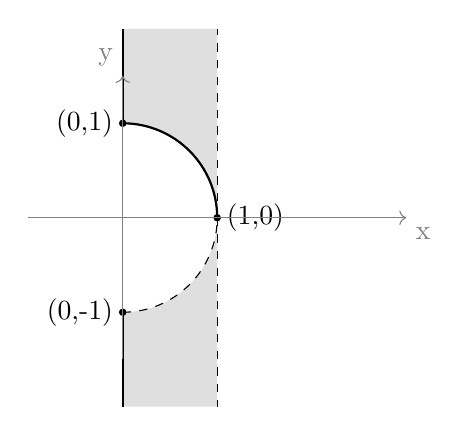
\begin{tikzpicture}[yscale=1.2, xscale=1.2]
            \fill[fill=gray!25] (0,-2) -- (0,-1) arc[start angle=270, end angle=360, radius=1] -- (1,0) -- (1,-2) -- cycle;
            \fill[fill=gray!25] (1,2) -- (1,0) arc[start angle=0, end angle=90, radius=1] -- (0,1) -- (0,2) -- cycle;
            \fill (1,0) circle (0.04);
            \node at (1,0) [right] {(1,0)};
            \fill (0,1) circle (0.04);
            \node at (0,1) [left] {(0,1)};
            \fill (0,-1) circle (0.04);
            \node at (0,-1) [left] {(0,-1)};
            \draw [thick] (0,1)--(0,2);
            \draw [thick] (0,-1)--(0,-2);
            \draw [thick] (0,1) arc (90:0:1);
            \draw [dashed] (1,0)--(1,2);
            \draw [dashed] (0,-1) arc (270:360:1);
            \draw [dashed] (1,0)--(1,-2);
            \draw[color=gray,->] (-1,0)--(3,0) node[anchor = north west] {x};
            \draw[color=gray,->] (0,-1.5)--(0,1.5) node[anchor = south east] {y};
        \end{tikzpicture}
    \end{center}

\end{solution}

\subsection{解析覆盖和模函数}

\begin{problem}{}
    证明任何 Riemann 曲面总存在解析万有覆盖。
\end{problem}
\begin{solution}
    利用万有覆盖存在定理(这里使用一个弱版本)。由于 Riemann 曲面 $S$ 连通而且局部道路连通且局部单连通。考虑如下路径空间
    \begin{equation*}
        \widetilde{S} := \{\gamma_{x}: \gamma:[0,1] \to S,\gamma(0) = x,\gamma(1) = y \in U_{x}\}
    \end{equation*}
\end{solution}

\begin{problem}{}
    证明覆盖变换群的性质1和性质2。
\end{problem}
\begin{solution}
1.离散性:反证法,如果有聚点 $\widetilde{z}^{*}$,那么在聚点的小邻域内都有
\begin{equation*}
    \pi^{-1}(\pi(\widetilde{z}^{*})) = \{\gamma(\widetilde{z}_{k}):\widetilde{z}_{k} \to \widetilde{z}^{*}\} \supsetneq \widetilde{z}^{*}
\end{equation*}
于是覆盖 $\pi$ 不是单射,与局部共形矛盾。\\
2.覆叠变换和覆叠次数的对应:如果 $\gamma $ 有不动点 $\widetilde{z_{0}}$ ,那么考虑覆盖映射 $\pi$ 对应的提升如下
\begin{center}
    \begin{tikzcd}
                & {(\widetilde{S},\widetilde{z_{0}})} \arrow[d, "\pi"] \\
        {(\widetilde{S},\widetilde{z_{0}})} \arrow[r, "\pi"] \arrow[ru, "\exists ! \gamma", dashed] & {(S,\pi(\widetilde{z_{0}}))}                         
    \end{tikzcd}
\end{center}
那么 $\gamma$ 和 $\mathrm{Id}_{\widetilde{S}}$ 都给出了上述交换图提升的解,根据覆盖空间的映射提升定理,提升是唯一的,只能有
\begin{equation*}
    \gamma = \mathrm{Id}_{\widetilde{S}}
\end{equation*}
\end{solution}
\begin{note}
    覆盖空间的映射提升的唯一性来自于拓扑,注意到在基点处覆盖映射是局部同胚,那么提升在此局部就被唯一确定。而 Riemann 面是道路连通空间,任何点都可以通过连续道路和基点相连,在这样的道路上考虑提升在局部的唯一性就给出结论。事实上也就是说将一个点映射到基点原象 $\pi^{-1}(x)$ 中的某点的提升都是唯一的。
\end{note}

\begin{problem}{}
    设 $\pi:\widetilde{S} \to S$ 是解析覆盖,$\Gamma$ 是覆盖变换群。求证 $\widetilde{S}/\Gamma$ 是 Riemann 曲面且共形等价于 $S$。
\end{problem}
\begin{solution}

\end{solution}

\begin{problem}{}
    设 $\pi:\widetilde{S} \to S$ 是解析万有覆盖,给定 $\widetilde{z_{0}} \in \widetilde{S},z_{0} = \pi(\widetilde{z_{0}})\in S$。证明对任何的 $\widetilde{z_{0}'} \in \pi^{-1}(z_{0})$ 存在唯一的覆盖变换 $\gamma$ 使得 $\gamma(\widetilde{z_{0}}) = \widetilde{z_{0}'}$。
\end{problem}
\begin{solution}
设 $\gamma_{1},\gamma_{2}$ 同时将 $\widetilde{z_{0}}$ 映射到 $\widetilde{z_{0}'}$ 则
\begin{equation*}
    \gamma_{2}^{-1}\gamma_{1}\widetilde{z_{0}}=\widetilde{z_{0}}
\end{equation*}
根据6.2.2的对应关系有 $\quad\gamma_{2}^{-1}\gamma_{1}=id$ 从而 $\gamma_{1} = \gamma_{2}$。
\end{solution}

\begin{problem}{}
    证明下列解析映射都是常值映射:
    \begin{equation*}
        (1)\, f:\mathbb{C}_{\infty}\to\mathbb{C};
        (2)\, f:\mathbb{C} \to \mathbb{C}_{0,1};
        (3)\, f:\mathbb{C}\setminus\{0\} \to \mathbb{C}_{0,1}
    \end{equation*}
\end{problem}
\begin{solution}
\begin{itemize}
    \item $f$ 在 $\infty$ 处解析相当于在坐标变换下 $f(\frac{1}{z})$ 在原点附近解析,也就是 $f$ 在 $\C-D(0,R)$ 外有界,事实上就是说明 $f|_{C}:\C \to \C$ 是有界解析函数,从而 $f$ 只能是常数。
    \item 我们已经知道 $\varphi:\mathbb{D}\to C_{0,1}$ 是覆盖映射,考虑映射提升 $\widetilde{f}:\mathbb{C}\to\mathbb{D}$ 结合 Liouville 定理得 $\varphi\circ \widetilde{f}=f$ 为常数。
    \item 考虑 $\C \xrightarrow{e^{2\pi \sqrt{-1}z}} \C - \{0\}$ 是解析覆盖,如果有 $f:\C-\{0\} \to \C_{0,1}$ 那么复合给出解析映射如
            \begin{equation*}
                \C \xrightarrow{e^{2\pi \sqrt{-1}z}} \C - \{0\} \xrightarrow{f} \C_{0,1}
            \end{equation*}
            根据上一项可知这只能是常数函数。
\end{itemize}
\end{solution}

\begin{problem}{}
    确定是否存在非常值解析映射 $f:\mathbb{C}_{0,1} \to \mathbb{D}$。
\end{problem}
\begin{solution}
    不存在。\\
    首先考虑 Riemann 可去奇点定理,也就是如果 $z_{0}$ 是解析函数 $f$ 的孤立奇点,而且 $f$ 在 $z_{0}$ 附近有界,则 $z_{0}$ 是 $f$ 的可去奇点。证明可以通过定义
    \begin{equation*}
        F(z) = 
        \begin{cases}
            (z-z_{0})^{2}f(z) & z\not= z_{0}\\
            0         & z=z_{0}\\
        \end{cases}
    \end{equation*}
    那么根据 $f$ 在 $z_{0}$ 附近有界,设 $f$ 在 $\Omega$ 上解析,那么此时 $F$ 在 $\Omega\cup \{z_{0}\}$ 上解析,而且
    \begin{equation*}
        F(z_{0}) = F'(z_{0}) = 0
    \end{equation*} 
    从而 $F(z) = (z-z_{0})^{2}h(z)$,这里 $h$ 是 $\Omega\cup \{Z_{0}\}$ 上的解析函数,显然 $h$ 是 $f$ 的解析延拓。于是 $z_{0}$ 是 $f$ 的可去奇点。
    如果存在解析函数 $f:\C_{0,1} \to \D$,根据 Riemann 可去奇点定理说明 $0,1$ 都是 $f$ 的可去奇点,从而其存在解析延拓
    \begin{equation*}
        \widetilde{f}:\C \to \D
    \end{equation*}
    那么根据 Liouville 定理只能有 $f$ 为常数。
\end{solution}

\section{第七章:双曲度量}

\subsection{单位圆上的Poincar\'e度量}

\begin{problem}{}
    验证(6.1)和(6.2)。
\end{problem}
\begin{solution}
    此时根据单位圆盘上的双曲距离表达式
    \begin{equation*}
        d_{\D}(z,z_{0}) = \ln(\frac{1+\delta(z,z_{0})}{1-\delta(z,z_{0})}),\quad \delta(z,z_{0}) = \frac{|z-z_{0}|}{|1-\overline{z_{0}}z|} 
    \end{equation*}
    当 $|z| \to 1$ 时,根据连续性
    \begin{equation*}
        1 + \delta(z,z_{0}) \le 2
    \end{equation*}
    而
    \begin{equation*}
        1 - \delta(z) = \frac{1}{1-|z|}
    \end{equation*}
    验证双曲圆是欧式圆只需要考察
    \begin{equation*}
        \delta(z,z_{0}) \le \frac{e^{R}-1}{e^{R}+1}
    \end{equation*}
    相当于集合。。。
\end{solution}

\begin{problem}{}
    在上半平面 $\mathbb{H}$ 上定义 Poincar\'e 度量。
\end{problem}
\begin{solution}
    利用共形映射 $\phi:\Hp \to \D$
    \begin{equation*}
        \phi(z) = \frac{z-\sqrt{-1}}{z+\sqrt{-1}}
    \end{equation*}
    保持双曲度量,那么
    \begin{equation*}
        \rho_{\Hp}(z) = \rho_{\D}(\phi(z))|\phi'(z)| = \frac{2|z+\sqrt{-1}|^{2}}{|z+\sqrt{-1}|^{2}-|z-\sqrt{-1}|^{2}}\frac{2}{|z+\sqrt{-1}|^{2}} = \frac{1}{\mathrm{Im}z}
    \end{equation*}
\end{solution}

\begin{problem}{}
    设 $\phi:\mathbb{D}\to\mathbb{C}_{0,1}$ 是模函数,取 $f:\mathbb{D} \to \mathbb{C}_{0,1}$ 解析且 $f(0) = \phi(0)$。证明对任何的 $0<r<1$
    \begin{equation*}
        \sup_{|z|\le r}|f(z)| \le \sup_{|z|\le r}|\phi(z)|
    \end{equation*}
\end{problem}
\begin{solution}
\end{solution}

\subsection{一般区域上的双曲度量}

\begin{problem}{提升映射保持测地性质}
    设 $f:\Omega_{1}\to\Omega_{2}$ 是解析覆盖映射,$\gamma$ 是 $\Omega_{2}$ 内关于双曲度量 $\rho_{\Omega_{2}}(z)|dz|$ 的一条测地线。证明 $\gamma$ 在 $\Omega_{1}$ 中的提升 $\widetilde{\gamma}$ 是 $\Omega_{1}$ 中关于双曲度量 $\rho_{\Omega_{1}}(\zeta)|d\zeta|$ 的测地线。
\end{problem}
\begin{solution}
记 $f:\Omega_{1}\to\Omega_{2},\zeta\to z$

取 $\Gamma$ 是连接 $z_1$ 和 $z_2$ 的曲线族有
\begin{equation*}
    \int_{\gamma}\rho_{2}(z)|dz|\leq \int_{\Gamma}\rho_{2}(z)|dz|
\end{equation*}
利用讲义定理6.6的 $\rho_{1}(\zeta)|d \zeta|=\rho_{2}(f(\zeta))|dz|$ 
代入得到
\begin{equation*}
    \int_{f^{-1}(\gamma)}\rho_{}(\zeta)|d\zeta|\leq \int_{f^{-1}(\Gamma)}\rho_{1}(\zeta)|d\zeta|
\end{equation*}
这给出 $\widetilde{\gamma}$ 是测地线(geodesic)。
\end{solution}

\begin{problem}{}
    设 $\Omega$ 是双曲区域并取定 $z_{0} \in \Omega$。证明对 $z\in\Omega,z\to\partial\Omega$ 都有 $d_{\Omega}(z,z_{0}) \to \infty$。
\end{problem}
\begin{solution}
根据上一题,选取测地线 $\gamma$ (depends on $z$) 并且提升映射到单位圆盘,于是
\begin{equation*}
    d_{\Omega}(z,z_0)=\int_{\gamma}\rho(z)|dz|=\int_{\widetilde{\gamma}}\frac{2|d\zeta|}{1-|\zeta|^{2}}
\end{equation*}
从而当 $z\to \partial\Omega,|\zeta|\to 1$ 有 $d_{\Omega}(z,z_0)\to\infty$.
\end{solution}

\begin{problem}{}
    验证例6.1中各区域的双曲度量的显式表达式。
\end{problem}
\begin{solution}
根据共形映射1,2,4是一类,根据 $e^{\sqrt{-1} z}:\mathbb{H}\to \mathbb{D}\setminus \{0\}$ 得到穿孔单位圆的双曲度量,再根据3得到5。
\end{solution}

\begin{problem}{}
    设 $\Omega \subset \mathbb{C}$ 是单连通双曲区域,证明对任何的 $z_1,z_2\in \Omega$ 都有
    \begin{equation*}
        |\ln \rho_{\Omega}(z_1) - \ln \rho_{\Omega}(z_2)| \le 2 d_{\Omega}(z_1,z_2)
    \end{equation*}
\end{problem}
\begin{solution}
问题转化到单位圆上计算双曲距离:
\begin{equation*}
    \ln \frac{\left(1-\left|\zeta_{2}\right|^{2}\right)\left|\varphi^{\prime}\left(\zeta_{2}\right)\right|}{\left(1-\left|\zeta_{1}\right|^{2}\right)\left|\varphi^{\prime}\left(\zeta_{1}\right)\right|} \leqslant 2d_{\mathbb{D}}\left(\zeta_{1}, \zeta_{2}\right)
\end{equation*}
取 $\zeta_1=0$ 用Koebe distortion theorem 估计 $\frac{\varphi^{\prime}(\zeta_2)}{\varphi^{\prime}(0)}$ 得到
\begin{equation*}
    \left|\frac{\phi'(\zeta_2)}{\phi'(0)}\right|
    \le \frac{1 + |\zeta_2|}{(1 - |\zeta_2|)^3}
\end{equation*}
给出
\begin{equation*}
     \ln \frac{\left(1-\left|\zeta_{2}\right|^{2}\right)\left|\varphi^{\prime}\left(\zeta_{2}\right)\right|}{\left(1-\left|\zeta_{1}\right|^{2}\right)\left|\varphi^{\prime}\left(\zeta_{1}\right)\right|}
     \le 2 \ln \frac{1+|\zeta_2|}{1-|\zeta_2|} \le 2d_{\D}(0,\zeta_2)
\end{equation*}
这里在双曲圆盘上采用的是经典度量
\begin{equation*}
    d_{\D}(z_1,z_2) := \ln R(z_1,z_2;w_1,w_2)
    = \ln\frac{|z_2 -w_1| |z_1 - w_2|}{|z_1 - w_1| |z_2 -W_2|}
\end{equation*}

\end{solution}

\begin{problem}{}
    设 $\Omega \subset \mathbb{C}$ 是单连通双曲区域,$\mathbb{D}_{\Omega}(z)=\{\zeta\in\Omega:d_{\Omega}(\zeta,z)<1\}$ 是以 $z$ 为中心的双曲圆,记 $\delta(z) = d(z,\partial\Omega)$ 是 $z$ 到 $\Omega$ 边界的欧式距离,$\mathrm{diam}\mathbb{D}_{\Omega}(z)$ 是 $\mathbb{D}_{\Omega}(z)$ 的欧式直径。证明存在常数 $0 < k_{1} < k_{2} < +\infty$ 使得
    \begin{equation*}
        k_{1}\delta(z) \le \mathrm{diam}\mathbb{D}_{\Omega}(z) \le k_{2}\delta(z)
    \end{equation*}
\end{problem}
\begin{solution}
\end{solution}

\begin{problem}{}
    设 $\Omega \subset \mathbb{C}$ 是单连通双曲区域,给定 $a\in\Omega$。设 $\phi:\Omega \to \mathbb{D},\phi(a) = 0$ 是 Riemann 映射:
    \begin{description}
        \item[(1)]  写出 $\Omega$ 上以 $a$ 为奇点的格林函数 $g$;
        \item[(2)]  设 $\Omega^{*} = \Omega -\{a\}$,求出 $\Omega^{*}$ 上的双曲度量 $\rho_{\Omega^{*}}(z)|dz|$;
        \item[(3)]  证明对于任何的 $z_{1},z_{2}\in \Omega^{*}$  
                    \begin{equation*}
                        d_{\Omega^{*}}(z_{1},z_{2}) \ge |\ln g(z_{1},a) - \ln g(z_{2},a)|
                    \end{equation*}
    \end{description}
\end{problem}
\begin{solution}
\end{solution}

\subsection{超双曲度量}

\begin{problem}{}
    求当 $z \in \Omega_{\infty}$ 时 $\rho_{0,1}(z)$ 的一个下界,并求出当 $z$ 趋于无穷时 $\rho_{0,1}(z)$ 的渐近行为。
\end{problem}
\begin{solution}
    
\end{solution}

\begin{problem}{}
    证明推论6.16。
\end{problem}
\begin{solution}
    
\end{solution}

\begin{problem}{}
    证明: $\C$ 和 $\C^{*}$ 上不存在超双曲度量.
\end{problem}
\begin{solution}
    
\end{solution}

\begin{problem}{}
    设 $\Omega \subset \C$ 是双曲区域 $\rho_{\Omega}(z)|dz|$ 是双曲度量,$\rho_{S}(z)|dz|$ 是球面度量,求证
    \begin{equation*}
        \lim_{z\to\zeta\in\partial\Omega}\frac{\rho_{\Omega}(z)}{\rho_{S}(z)} = \infty
    \end{equation*}
    这里 $\partial \Omega$ 包含无穷远点。
\end{problem}
\begin{solution}
\end{solution}

\begin{problem}{}
    设 $\Omega \subset \C$ 是双曲区域 $D_{Ω}(z) $ 是 $\Omega$ 内以 $z$ 为圆心的双曲单位圆, 记 $\mathrm{diam}_{S}D_{Ω}(z)$ 是 $D_{Ω}(z)$ 在球面距离下的直径。则
    \begin{equation*}
        \lim_{z\to \partial\Omega}\mathrm{diam}_{S}D_{Ω}(z) = 0
    \end{equation*}
\end{problem}
\begin{solution} 
\end{solution}

\begin{problem}{}
    利用Schottkey定理证明Picard小定理。
\end{problem}
\begin{solution}
\end{solution}


\section{第八章:Riemann zeta函数}

\begin{problem}
    证明
    \[
    \ln \zeta(s)  = \sum_{p,m}\frac{p^{-ms}}{m}
    \]
\end{problem}

\begin{solution}
    根据欧拉乘积和泰勒展开 $\ln(1+x) = \sum_{n\ge 1} (-1)^{n-1}\frac{x^n}{n}$ 形式计算
    \begin{align*}
        \ln \zeta (s) &= \ln \prod_{p}\frac{1}{1-p^{-s}} = \sum_p - \ln(1- p^{-s})\\
        & = \sum_{p,m} \frac{p^{-ms}}{m}
    \end{align*}
    收敛性由于 $|\mathrm{Re}s|>1$ 得到。
\end{solution}

\section{补充题目}

\begin{problem}{2012-26}
    如果 $\Omega$ 是一个共形等价于 $A(R_{1},R_{2})$ 的区域,那么取其有限余分支是 $D_{2}$,其无界余分支的补集记成 $D_{1}$ 则
    \begin{equation*}
        \frac{\mathrm{A}(D_{1})}{\mathrm{A}(D_{2})} \ge \frac{R_{2}^{2}}{R_{1}^{2}}
    \end{equation*}
    等号成立当且仅当 $\Omega = A(R_{1},R_{2})$。而且有如下面积不等式
    \begin{equation*}
        \mathrm{A}(D_{2}) \le \frac{\mathrm{A}(D_{1})}{e^{\pi (\ln R_{2}-\ln R_{1})}-1}
    \end{equation*}
\end{problem}
\begin{solution}
    
\end{solution}

\end{document}